\documentclass[10pt]{report}
\usepackage{amssymb}
\usepackage{graphicx}
\usepackage{makeidx}

\setcounter{secnumdepth}{4}


\newcommand{\ens}[4]{ {#1}_{\mathbb{#2}} \leftarrow {#3}_{\mathbb{#4}} }



\def\applyTrsf{\texttt{applyTrsf}\index{applyTrsf@\texttt{applyTrsf}} } 
\def\applyTrsfToPoints{\texttt{applyTrsfToPoints}\index{applyTrsfToPoints@\texttt{applyTrsfToPoints}} }
\def\baladin{\texttt{baladin}\index{baladin@\texttt{baladin}} }
\def\blockmatching{\texttt{blockmatching}\index{blockmatching@\texttt{blockmatching}} }
\def\buildPyramidImage{\texttt{buildPyramidImage}\index{buildPyramidImage@\texttt{buildPyramidImage}} }
\def\composeTrsf{\texttt{composeTrsf}\index{composeTrsf@\texttt{composeTrsf}} }
\def\copyTrsf{\texttt{copyTrsf}\index{copyTrsf@\texttt{copyTrsf}} }
\def\createGrid{\texttt{createGrid}\index{createGrid@\texttt{createGrid}} }
\def\createTrsf{\texttt{createTrsf}\index{createTrsf@\texttt{createTrsf}} }
\def\cropImage{\texttt{cropImage}\index{cropImage@\texttt{cropImage}} }
\def\invTrsf{\texttt{invTrsf}\index{invTrsf@\texttt{invTrsf}} }
\def\pointmatching{\texttt{pointmatching}\index{pointmatching@\texttt{pointmatching}} }
\def\printImage{\texttt{printImage}\index{printImage@\texttt{printImage}} }
\def\printTrsf{\texttt{printTrsf}\index{printTrsf@\texttt{printTrsf}} }

\newenvironment{attention}{\begin{description}\item[{[\textsc{Pay attention}]}]}{\end{description}}
%\newenvironment{attention}{\noindent \textsc{[Pay attention]}}{}
% \def\attention{\textsc{[Pay attention]} }

\newenvironment{note}{\begin{description}\item[{[\textsc{Note:}]}]}{\end{description}}
% \newenvironment{note}{\noindent \textsc{[Note]}}{}
% \def\note{\textsc{[note]} }


\newcommand{\option}[1]{{\texttt{'#1'}}}

\newenvironment{code}[1]{\mbox{}\\[1ex]\hspace*{-#1cm}\begin{minipage}{150mm}\begin{quote}\tt}{\end{quote}\end{minipage}\mbox{}\\[1ex]}

%\newenvironment{code}[1]{\mbox{}\\[1ex]\begin{minipage}{150mm}\tt}{\end{minipage}\mbox{}\\[1ex]}


\makeindex

\begin{document}

\title{\texttt{blockmatching} and associated tools, a very short documentation}
\author{Gr\'egoire Malandain}
\maketitle

\tableofcontents



\part{User documentation}


\chapter{Command Line Interfaces}





\section{\blockmatching}
\label{sec:blockmatching}

\subsection{Basic use}

\blockmatching registers a floating image $I_{flo}$ onto a reference image $I_{ref}$, and yields two results: the transformation from the reference image frame towards the floating image frame,  $T_{res} = T_{I_{flo} \leftarrow I_{ref}}$, and the floating image resampled in the same frame than the reference image, $I_{res} = I_{flo} \circ T_{I_{flo} \leftarrow I_{ref}}$.

\begin{code}{0.8}
\% \blockmatching -flo $I_{flo}$ -ref $I_{ref}$ -res $I_{res}$ -res-trsf $T_{res}$ ...
\end{code}

$T_{res} = T_{I_{flo} \leftarrow I_{ref}}$ allows to resample $I_{flo}$, or any image defined in the same frame than $I_{flo}$, into the same frame than $I_{ref}$, which can also be done afterwards with \applyTrsf.

\begin{code}{0.8}
\% \applyTrsf $I_{flo}$ $I_{res}$ -trsf $T_{res}$ -template $I_{ref}$
\end{code}

For instance, this allows to \textit{visualize} the deformation undergone by $I_{flo}$ by applying the transformation to a grid image (see \createGrid). 





\subsection{Principle}

The principle of \blockmatching is to pair blocks from the floating
image $I_{flo}$ with blocks of the  reference image $I_{ref}$,
i.e. for each blocks in  the floating
image $I_{flo}$, we are looking in a neighborhood of the reference
image $I_{ref}$ for the best similar block.

More precisely, \blockmatching computes $T_{res} = T_{I_{flo} \leftarrow I_{ref}}$ that allows to resample $I_{flo}$ in the frame of $T_{ref}$.
At iteration $i$, pairings are built between $I_{flo} \circ T^{(i)}_{I_{flo} \leftarrow I_{ref}}$ ($I_{flo}$ resampled by the estimation of $T_{I_{flo} \leftarrow I_{ref}}$ at iteration $i$) and $T_{ref}$. With these pairings, an incremental transformation $\delta T^{(i)} = T_{I^{(i)}_{flo} \leftarrow I_{ref}}$ is computed and used to update the transformation:
\begin{displaymath}
T^{(i+1)}_{I_{flo} \leftarrow I_{ref}} 
= T^{(i)}_{I_{flo} \leftarrow I_{ref}} \circ \delta T^{(i)}
\end{displaymath}

\begin{itemize}

\item Registration can be conducted within a hierarchical approach, by the means of image pyramids: see section \ref{sec:parameters:hierarchical}.

\item Pairings are built by associating similar blocks (or small images) between the resampled floating image $I_{flo} \circ T^{(i)}_{I_{flo} \leftarrow I_{ref}}$ and the reference image $I_{ref}$: section \ref{sec:parameters:block:definition} introduces some option for the block definition while section \ref{sec:parameters:block:pairing} presents options for block pairings.

\item Transformations are estimated by the means of (weighted) least (trimmed) squares: see section \ref{sec:parameters:transformation:estimation} for generic options for transformation estimation, and section \ref{sec:parameters:vectorfield:estimation} that presents dedicated options for vector field estimation.

\end{itemize}






\subsection{Options and parameters (general informations)}


Running the program without any options gives the minimal syntax:
\begin{code}{1}
\% \blockmatching 
\end{code}
Running it with either \option{-h} or \option{--h} gives the option list:
\begin{code}{1}
\% \blockmatching -h
\end{code}
Running it with either \option{-help} or \option{--help} gives some details about the options:
\begin{code}{1}
\% \blockmatching -help
\end{code}

\begin{attention} 
Default parameters depend on the transformation type (linear or non-linear). 
The \option{-print-parameters} allows printing the values of the parameters, so running \blockmatching with this option along with the chosen type of transformation (with \option{-trsf-type}) may be a good idea. 
\begin{code}{1}
\% \blockmatching ... -print-parameters
\end{code}
If a logfile name is given (with option \option{-logfile}), parameter values will be printed out in this file.

In addition, when changing parameters, comparing the parameter values with the \option{-print-parameters} before and after the parameter changes allows to check that the applied changes are the expected ones.
\end{attention}










\subsection{Initial transformations}
Two transformations, $T_{left}$ and $T_{init}$, can be passed
as parameters. While $T_{left}$ (left-handed transformation) will remain unchanged during the
registration procedure, $T_{init}$ is the initial value of the
transformation to be computed (recall this is an iterative
calculation). More precisely (see also section~\ref{sec:field:view:center:alignment}), let $T^{(0)}$ denote the initial value
the transformation to be computed.

\begin{itemize}
\item if $T_{init}$ is given, $T^{(0)} = T_{init}$ 
\item else 
\begin{itemize}
\item if $T_{left}$ is given, $T^{(0)}  = \mathbf{Id}$
\item else (neither $T_{init}$ nor $T_{left}$ are given), $T^{(0)}$ is the default transformation (can be specified with the \option{-default-transformation} option). It is either the translation that superimposes the centers of the fields of view of the two images $I_{ref}$ and $I_{flo}$ (\option{-default-transformation fovcenter}),  or the identity (\option{-default-transformation identity}). 
The default behavior is to superimpose the centers of field of view (see section \ref{sec:field:view:center:alignment}).
\end{itemize}
\end{itemize}

The initial state of the registration procedure is the
comparison of the reference image $I_{ref}$ with the transformed
floating  image $I_{flo} \left( \circ T_{left} \right) \circ T^{(0)}$.
\begin{itemize}
\item[] \option{-[left|initial]-transformation} allows to initialize $T_{left}$, while
\item[] \option{-initial-result-transformation} allows to initialize $T_{init}$
\end{itemize}

\begin{itemize}

\item the option \option{-[initial|left]-[voxel-]transformation} is
  used to specify a transformation $T_{left}$ that is applied to the
  floating image $I_{flo}$. Therefore, it comes to register $I_{flo}
  \circ T_{left}$ with $I_{ref}$. Thus, the resulting transformation,
  $T_{res}$, allows to resample $I_{flo}$ onto $I_{ref}$ by
  calculating $I_{flo} \circ T_{left} \circ T_{res}$.

In other words, the transformation $T_{res}$ obtained with
\begin{code}{1}
\% \blockmatching -flo $I_{flo}$ -ref $I_{ref}$ ... -initial-transformation $T_{left}$  -res-trsf $T_{res}$
\end{code}
is comparable to the one, $T_{res,2}$ obtained with the following commands
\begin{code}{1}
\% \applyTrsf $I_{flo}$ $I_{flo,2}$ -trsf $T_{left}$ \\
\% \blockmatching -flo $I_{flo,2}$ -ref $I_{ref}$ ... -res-trsf $T_{res,2}$
\end{code}

\begin{note}
When the \option{-composition-with-[initial|left]} is specified, the
result transformation that is written is $T_{left} \circ T_{res}$. 
\end{note}

This may be useful in case of successive registrations, e.g. with
different transformation types. Indeed, one may want to first register
the two images $I_{flo}$ and $I_{ref}$ with a rigid transformation and
then with an affine transformation.

\begin{enumerate}
\item A first solution is to compute the rigid transformation
\begin{code}{1}
\% \blockmatching -flo $I_{flo}$ -ref $I_{ref}$ ... -res-trsf
$T_{rig}$ -trsf-type rigid -res $I_{flo,2}$
\end{code}
and then an affine transformation by comparing the previous result
$I_{flo,2} = I_{flo} \circ T_{rig}$ with $I_{ref}$
\begin{code}{1}
\% \blockmatching -flo $I_{flo,2}$ -ref $I_{ref}$ ... -res-trsf
$T_{aff}$ -trsf-type affine -res $I_{flo,3}$
\end{code}
$I_{flo}$ can be then be directly resampled onto $I_{ref}$ with the
composed transformation $T_{resampling} = T_{rig} \circ T_{aff}$
\begin{code}{1}
\% \composeTrsf -res $T_{resampling}$ -trsfs $T_{rig}$ $T_{aff}$
\end{code}

\item A second solution consists in also first computing the rigid transformation
\begin{code}{1}
\% \blockmatching -flo $I_{flo}$ -ref $I_{ref}$ ... -res-trsf
$T_{rig}$ -trsf-type rigid -res $I_{flo,2}$
\end{code}
but then $T_{rig}$ is used as parameter to
\option{-left-transformation} with $I_{flo}$ as floating image
\begin{code}{1}
\% \blockmatching -flo $I_{flo}$ -ref $I_{ref}$ ... -res-trsf
$T_{aff}$ -trsf-type affine -res $I_{flo,4}$ -left-transformation $T_{rig}$
\end{code}
This second solution is to be prefered. Indeed, the resampled version of
$I_{flo}$ by $T_{rig}$ can miss some data (data of $I_{flo}$ that are
not in the field of view (FOV) of $I_{ref}$ after resampling) and
cropping effects may appear (parts of FOV of  $I_{ref}$ that do not
have correspondant areas in  $I_{flo}$ by $T_{rig}$).

Note that the command
\begin{code}{1}
\% \blockmatching -flo $I_{flo}$ -ref $I_{ref}$ ... -res-trsf
$T_{resampling}$ -trsf-type affine -res $I_{flo,4}$ -left-transformation
$T_{rig}$ -composition-with-left
\end{code}
has $T_{resampling}$ as output transformation.

\end{enumerate}

\item \label{opt:initial:result:transformation} the option \option{-initial-result-[voxel-]transformation} is used to specify the initial value of the transformation to be computed. This can be used to continue a registration done at the higher scale.

For instance, the result transformation $T_{res}$ computed in one shot by
\begin{code}{1}
\% \blockmatching -flo $I_{flo}$ -ref $I_{ref}$ ...  -res-trsf
$T_{res}$ -py-ll 0 -py-hl 3 -flo-frac 0.75
\end{code}
is equal to the result transformation $T_{res,2}$ that is computed in two step (the first step uses the scales 3 and 2, while the second one uses the scales 1 and 0).
\begin{code}{1}
\% \blockmatching -flo $I_{flo}$ -ref $I_{ref}$ ...  -res-trsf
$T_{intermediary}$ -py-ll 2 -py-hl 3 -flo-frac 0.75 \\
\% \blockmatching -flo $I_{flo}$ -ref $I_{ref}$ ...  -init-res-trsf
$T_{intermediary}$ -res-trsf $T_{res,2}$ -py-ll 0 -py-hl 1 -flo-frac 0.75
\end{code}
This may allow to qualitatively evaluate the intermediary result before running the algorithm at the lower scales that are computationaly expensive.

\begin{note}
Please note the \option{-flo-frac 0.75} (see option
\option{-floating-selection-fraction}, page
\pageref{opt:floating:selection:fraction}) that sets the fraction of
blocks of the floating image to be kept for the pairing search. Thanks
to this option, it is constant through the pyramid levels, and for
both computation schemes (one-step and two-steps).
\end{note}

\end{itemize}

Initial transformations can be obtained by pairing points with \pointmatching (see section \ref{sec:pointmatching}).



\subsection{Result transformation}

\option{-result-[voxel-]transformation} is used to specify the name of
the output transformation.

When no left-handed transformation is passed, it is the transformation $T_{res} = T_{I_{flo} \leftarrow
  I_{ref}}$ that allows to resample $I_{flo}$ onto $I_{ref}$.

When a left-handed transformation is passed with the option
\option{-left-[voxel-]transformation}, the result transformation $T_{res}$ is
the one that allows to resample  $I_{flo} \circ T_{left}$ onto
$I_{ref}$, i.e. $T_{res} = T_{I_{flo} \circ T_{left} \leftarrow
  I_{ref}}$. 
%
This should be the default behavior that can
be enforced with the option \option{-no-composition-with-left}.
%
To resample directly $I_{flo}$ onto $I_{ref}$, it is required to have
$T_{left} \circ T_{res}$ at hand. While it is straightforward to
compute it thanks to \composeTrsf, it is also possible to get the
composed transformation $T_{left} \circ T_{res}$ as the output
transformation with the option \option{-composition-with-left}.


\subsection{Some useful parameters}

The use of some parameters is detailed here. For a complete list of parameters (and short description of them), the user is advised to use the \option{-help} option.

\subsubsection{Hierarchical registration}
\label{sec:parameters:hierarchical}

To speed up the computation and to handle large deformations, the transformation is computed hierarchically. For each image 
$I_{flo}$ and $I_{ref}$, pyramids of images are built, i.e. the pyramid $\{I^n_{flo}, \ldots, I^0_{flo}\}$ for the $I_{flo}$ image, where $I^0_{flo} = I_{flo}$ and where the dimensions of $I^{i+1}_{flo}$ are the ones of $I^{i}_{flo}$ divided\footnote{This is not strictly true, since the dimensions of $I^1_{flo}$ will be chosen to be the $2^k$ values that are closest (and smaller) to  $I^0_{flo}$ dimensions when $I^0_{flo}$ dimensions are not powers of 2.} by 2.

Thus, the registration is done with pyramids
$\{I^h_{flo}, \ldots, I^l_{flo}\}$ and $\{I^h_{ref}, \ldots, I^l_{ref}\}$, with $h$ and $l$ respectively specified by the 
\option{-pyramid-highest-level} and 
\option{-pyramid-lowest-level} options. A first transformation is computed with $\{I^h_{flo},I^h_{ref}\}$, that is used as initialization for the registration of  $\{I^{h-1}_{flo},I^{h-1}_{ref}\}$, and so on and so forth until $\{I^l_{flo},I^l_{ref}\}$.

The lowest level of the pyramid (i.e. the image at its native sizes) is specified by $0$, i.e. \option{-pyramid-lowest-level 0}.

\begin{itemize}
\item Specifying a high value of $h$ allows to search for long-range pairings (since a small displacement at a high scale image corresponds to a large displacement at a lower scale), and to speed up the computation: for 3D images, the data are reduced with a factor 8 between two consecutive scales (and so is the number of blocks).
\item On the other hand, when looking for small deformations, specifying a large $h$ is definitively not adequate, except if the search neighborhood size is adapted to the scale.
\end{itemize}

The finest the resolution, the more heavy the computation. When it comes to tune parameters, it may be useful to only perform the registration with the highest levels of the pyramid (ie to specify a high value to the \option{-pyramid-lowest-level} option, and to visually check the results before launching the computation with the lowest levels of the pyramid.

Moreover, if the images to be registered are quite large, I/0 operations and pyramid computation can be quite costly. It may then be considered to compute subsampled images beforehand, either by choosing the subsampling parameters with \applyTrsf (see section \ref{sec:applyTrsf}) or by picking one of the pyramid images built with \buildPyramidImage (see section \ref{sec:buildPyramidImage}) that can be computed also beforehand, and then perform the registration on subsampled images. It is detailed in section \ref{sec:hand:made:hierarchical:registration}.





\subsubsection{Block definition/selection parameters}
\label{sec:parameters:block:definition}


To build blocks, two parameters are important:
\begin{itemize}
\item[] \option{-block-size} allows to specify the size of the blocks. Small blocks require a small computational effort to be processed (since the similarity measure complexity depends on the number of points inside the block), but are more likely to be paired to the "wrong" block. 

On the contrary, since the information distribution is more complex in a large block, pairing large blocks is more likely to build the "right" pairings
\item[] \option{-block-spacing} specify the spacing between consecutive blocks. Increasing the spacing allows to speed up the computation (by decreasing the number of blocks), at the price of sparser pairings. 
\end{itemize}

Some of the built blocks can be discarded for the pairing search, either because they may not yield pertinent pairings, or because they are not carrying useful information.

A first selection of points or blocks can be done based on intensity values, which may be useful to prevent blocks to be build in low intensity areas as the background.

\begin{itemize}
\item[] \option{-floating-low-threshold} and \option{-floating-high-threshold} allow to specify two intensity thresholds for the blocks built from the floating image $I_{flo}$. Points with values lower or equal to the low threshold, or higher or equal to the high threshold are discarded from the block for the similarity measure computation. 

\option{-floating-removed-fraction} specifies the maximal fraction of points that can be removed from a block. If too many points are removed (because of the two thresholds), the block is discarded and not considered for further computation.

\item[] options \option{-reference-low-threshold},\option{-reference-high-threshold}, and \option{-reference-removed-fraction} are similar options for the reference image $I_{ref}$.

\end{itemize}

Previous options help to control the building of individual blocks. To further control the total number of blocks (and hence decrease the computational effort), it is also possible to select the most informative blocks from the block list. According that the standard deviation is representative of the information (blocks of uniform values have a small standard deviation), the percentage of blocks of higher standard deviation can be specified, and only these blocks are considered for the transformation computation.

\begin{itemize}
\item[] \label{opt:floating:selection:fraction} \option{-floating-selection-fraction} allows to specify the fraction of blocks of the floating image to be kept for the pairing search. It can be more finely tuned with the suffixes \option{-ll} et \option{-lt}. 

\option{-floating-selection-fraction-ht} and
\option{-floating-selection-fraction-lt}  allow to specify this
fraction for respectively the highest and the lowest level of the
pyramid (see section \ref{sec:parameters:hierarchical}) while the
fraction value for intermediary levels is linearly interpolated from
these two fractions.

While it may not be required (even not advised) to remove blocks of
the floating image for the pairing search (and thus for the
transformation computation) at highest levels of the pyramid (where
there are few blocks), it may be convenient (even advised) to remove
some of them ar the lowest levels (where areas of constant image
intensity are likely to occur). Thus, default values for this fraction
are set to 1.0 for the highest level and 0.5 for the lowest level,
independently of the level values. This has to be kept in mind when
registration is conducted in several steps through the pyramid levels
(see option \option{-initial-result-transformation} page \pageref{opt:initial:result:transformation}).
\end{itemize}


\subsubsection{Block search/pairing}
\label{sec:parameters:block:pairing}

To build pairings, each (selected) block of the floating image is compared to blocks of the reference image, and is paired with its best correspondent. The comparison is restricted to a neighbourhood.
 
\begin{itemize}
\item[] \option{-search-neighborhood-half-size} allows to specify the size of the search neighbourhood (in the reference image for a given block from the floating image) to build pairings. The larger the value, the larger the searched displacement (and the larger the potential resulting deformation),  and, of course, the larger the computational effort.

\item[] \option{-search-neighborhood-step} allows to specify the step (the increment) between blocks in the search neighbourhood. Typically, a step equal to 2 allows to decrease by a factor 4 in 2D (8 in 3D) the number of blocks to tested in the search neighbourhood. However, the resulting pairings will be less precise.

\end{itemize}



\subsubsection{Transformation estimation}
\label{sec:parameters:transformation:estimation}

\begin{itemize}

\item[] \option{-transformation-type} allows to specify the type of computed transformation.It is desirable to compute transformation in a hierarchical manner, from the ones with few degrees of freedom to the ones with more degrees of freedom: e.g. \option{rigid}, then \option{affine}, then \option{vectorfield}.

\item[] \option{-estimator-type} allows to specify the calculation method to estimate the incremental transformation $\delta T$ from the pairings. Calculation is done by the mean of (weighted) least (trimmed) square. In case of weighted least (trimmed) squares, residuals to be minimized are weighted by the block similarity. Least trimmed squares methods allow to discard outliers from the transformation estimation.

\item[] Least trimmed squares estimation is an iterative method. At each iteration (except the first one where least squares estimation is used), outliers are discarded. Outliers are defined as the samples having the largest residuals after the previous estimation.

\option{-lts-fraction} defines the fraction of samples to be kept for estimation. Obviously, it should be larger than \option{0.5}.

\option{-lts-deviation} allows to define the outliers with respect to residual statistics (according they follows a normal law). Let $\hat{m}_r$ and $\hat{\sigma}_r$ be respectively the mean and the standard deviation of the residuals, passing the value $c$ to \option{-lts-deviation} set the residual rejection threshold at $\hat{m}_r + c \hat{\sigma}_r$.

\option{-lts-iterations} set a maximum number of iterations for the least trimmed squares estimation.


\end{itemize}



\subsubsection{Vector field transformations}
\label{sec:parameters:vectorfield:estimation}

Non-linear transformations are (up to today) encoded through vector fields. At each iteration $i$, an incremental transformation $\delta T$ est computed from the pairings, and then composed with the current transformation $T^i$ to yield the updated transformation $T^{i+1}$: 



\begin{itemize}
\item[] Building a vector field from pairing is done by interpolation with a Gaussian kernel whose standard deviation is specified by the \option{-fluid-sigma} option. Indeed, this interpolation also regularizes the pairings, and it can viewed as a fluid regularization since it is done on the incremental transformation.  It can be more finely tuned with the suffixes \option{-ll} et \option{-lt}. 

Note that the outliers detection (and removal) of trimmed estimations is done by comparing the pairings to the regularized $\delta T$.

\item[] \option{-elastic-sigma} is used afterwards (after composition with the incremental transformation) to regularize the global transformation $T^{i+1}$.

\item[] \option{-vector-propagation-distance} and \option{-vector-fading-distance} are presented in the section dedicated to \pointmatching (section \ref{sec:pointmatching}). They are more useful in case of (very) sparse pairings.

\end{itemize}





\subsection{Hints}

\subsubsection{How to tune parameters}

\begin{itemize}

\item A priori, pairings can be better built (and outliers can be better avoided) by specifying larger blocks with \option{-block-size} 

\item Non-informative (i.e. almost of uniform value) blocks should be avoided since they may yield poor pairings. Selection can be done either on point-wise criteria (e.g. intensity based selection with \option{-floating-low-threshold} and \option{-floating-high-threshold}) or block-wise criteria (e.g. \option{-floa\-ting-selection-fraction}).

\item When looking for small displacements/deformations, long distance pairings may be discouraged by
\begin{itemize}
\item only considering low levels of the pyramid (\option{-pyramid-highest-level}),
\item diminishing the size of the search neighbourhood (\option{-search-neigh\-borhood-half-size})
\end{itemize} 

\item The regularization of non-linear deformations can be tuned with both \option{-fluid-sigma}  and \option{-elastic-sigma}. The larger the values, the less local the deformations.

\end{itemize}


\subsubsection{Hand-made hierarchical registration}
\label{sec:hand:made:hierarchical:registration}


If the images to be registered are quite large, I/0 operations and pyramid computation can be quite costly. It may then be considered to compute subsampled images beforehand, either by choosing the subsampling parameters with \applyTrsf (see section \ref{sec:changing:image:geometry}) or by picking one of the pyramid images (see section \ref{sec:buildPyramidImage}) that can be computed also beforehand, and then perform the registration on subsampled images. 
In both case, it is mandatory to use \option{-res-trsf} to get the subsampling transformation.

Let us consider the images $I_{flo}$ and $I_{ref}$ to be registered. $I_{flo}$ can be subsampled into $I^s_{flo}$ with:
\begin{code}{0.8}
\% \applyTrsf $I_{flo}$ $I^s_{flo}$ $\ldots$ -res-trsf $T^s_{flo}$ -resize
\end{code}
and we get $I^s_{flo} = I_{flo} \circ T^s_{flo}$. The same stands for $I_{ref}$ and we get $I^s_{ref} = I_{ref} \circ T^s_{ref}$. Registration can be done on subsampled images with
\begin{code}{0.8}
\% blockmatching -flo $I^s_{flo}$ -ref $I^s_{ref}$ -res $I^s_{res}$ -res-trsf $T^s_{res}$ $\ldots$
\end{code}
$I^s_{res} = I^s_{flo} \circ T_{res}$ is $I^s_{flo}$ resampled in the geometry of $I^s_{ref}$. We have then
\begin{eqnarray*}
I^s_{res} = I^s_{flo} \circ T_{res}
& \Rightarrow &
I_{res} \circ T^s_{ref} = I_{flo} \circ T^s_{flo} \circ T_{res} \\
& \Rightarrow &
I_{res} = I_{flo} \circ T^s_{flo} \circ T^s_{res} \circ {T^s_{ref}}^{(-1)}
\end{eqnarray*}
A transformation $\tilde{T}_{res}$ that allows to transform $I_{flo}$ in the frame of $I_{ref}$ can be estimated by
$\tilde{T}_{res} = T^s_{flo} \circ T^s_{res} \circ {T^s_{ref}}^{(-1)}$, then with the commands
\begin{code}{0.8}
\% invTrsf  $T^s_{ref}$ ${T^s_{ref}}^{(-1)}$ \\
\% composeTrsf -res $\tilde{T}_{res}$ -trsfs $T^s_{flo}$ $T^s_{res}$ ${T^s_{ref}}^{(-1)}$ -template $I_{ref}$
\end{code}
$\tilde{T}_{res}$ can be calculated. Please notice the use of \option{-template} that ensures that  $\tilde{T}_{res}$  is defined on the $I_{ref}$ frame (mandatory for non-linear transformations).
Last, 
\begin{code}{0.8}
\% applyTrsf $I_{flo}$ $\tilde{I}_{res}$ -trsf  $\tilde{T}_{res}$ -template $I_{ref}$
\end{code}
yields $\tilde{I}_{res}$, ie $I_{flo}$ resampled in $I_{ref}$ frame thanks to $\tilde{T}_{res}$.

This is exemplified in section \ref{sec:example:applyTrsf:blockmatching}.



\section{\blockmatching versus \baladin}

% \subsection{Transformations}

A typical call to \blockmatching is
\begin{code}{0.8}
\% \blockmatching -flo $I_{flo}$ -ref $I_{ref}$ -res $I_{block}$ 
   -res-trsf $T_{block}$ -res-voxel-trsf $\hat{T}_{block}$ ...
\end{code}
where $I_{block}$, $T_{block}$, and $\hat{T}_{block}$ denote respectively the result image, i.e. the floating image resampled in the frame of $I_{ref}$, the transformation result in \textit{real} coordinates that allows to goes from $I_{ref}$ frame towards $I_{flo}$ frame (and then to resample $I_{flo}$ in the frame of $I_{ref}$), and the transformation result in \textit{voxel} coordinates.

A typical call to \baladin is
\begin{code}{0.8}
\% \baladin -flo $I_{flo}$ -ref $I_{ref}$ -res $I_{balad}$ 
-result-matrix $\hat{T}_{balad}$ -result-real-matrix $T_{balad}$ ...
\end{code}
where $I_{balad}$, $T_{balad}$, and $\hat{T}_{balad}$ denote respectively the result image, i.e. the floating image resampled in the frame of $I_{ref}$, the transformation result in \textit{real} coordinates that allows to goes from $I_{flo}$ frame towards $I_{ref}$ frame, and the transformation result in \textit{voxel} coordinates.

\begin{attention} The result transformation of \baladin is then the inverse of that of \blockmatching. We have 
$$ T_{block} \sim T^{-1}_{balad} \quad \mbox{ and } \quad \hat{T}_{block} \sim \hat{T}^{-1}_{balad}
$$
\end{attention}

Therefore $T_{block} \circ T_{balad}$ and $\hat{T}_{block} \circ \hat{T}_{balad}$ should be close to the identity, and this can be verified by computing $T_{test} = T_{block} \circ T_{balad}$
and $\hat{T}_{test} = \hat{T}_{block} \circ \hat{T}_{balad}$:
\begin{code}{0.8}
\% \composeTrsf -res $T_{test}$ -trsfs $T_{block}$ $T_{balad}$ \\
\% \printTrsf $T_{test}$\\
\% \composeTrsf -res $\hat{T}_{test}$ -trsfs $\hat{T}_{block}$ $\hat{T}_{balad}$\\
\% \printTrsf $\hat{T}_{test}$
\end{code}

The transformations issued from \baladin can be used to resample the floating image $I_{flo}$ but require to be inverted beforehand. To compute the resampled floating image $I_{balad}$ from the \textit{real} transformation $T_{balad}$, the commands are:
\begin{code}{0.8}
\% \invTrsf $T_{balad}$ $T^{-1}_{balad}$ \\
\% \applyTrsf $I_{flo}$ $I_{balad}$ -template $I_{ref}$ -trsf $T^{-1}_{balad}$
\end{code}
$I_{balad}$ can also be computed from from the \textit{voxel} transformation $\hat{T}_{balad}$ accordingly
\begin{code}{0.8}
\% \invTrsf $\hat{T}_{balad}$ $\hat{T}^{-1}_{balad}$ \\
\% \applyTrsf $I_{flo}$ $I_{balad}$ -template $I_{ref}$ -voxel-trsf $\hat{T}^{-1}_{balad}$
\end{code}










%%%%%%%%%%%%%%%%%%%%%%%%%%%%%%%%%%%%%%%%%%%%%%%%%%%%%%%%%%%%
%
%
%
%%%%%%%%%%%%%%%%%%%%%%%%%%%%%%%%%%%%%%%%%%%%%%%%%%%%%%%%%%%%










\section{\applyTrsf}
\label{sec:applyTrsf}

\subsection{Basic use}

\applyTrsf allows to resample an image according to a transformation $T$. One has to recall that the transformation goes from the \textit{destination/result image} towards the \textit{image to be resampled}. This is counter-intuitive, but can easily be explained: to compute the value of the point $M$ in the destination/result image, one has to know where this point comes from in the image to be resampled.

So, to resample the image $I_{flo}$ in the same frame than the image $I_{ref}$ with a transformation that $T$ goes from $I_{ref}$ towards $I_{flo}$, i.e. 
\begin{eqnarray*}
T & = & T_{I_{flo} \leftarrow I_{ref}} \\
I_{res} & = & I_{flo} \circ T
\end{eqnarray*}
 the command is  

\begin{code}{0.8}
\% \applyTrsf $I_{flo}$ $I_{res}$ -trsf $T$ -template $I_{ref}$
\end{code}

The \option{-trsf} implies that the transformation is in \textit{real frames} (i.e. the coordinates of the points are in real units, for instance millimeters). We recall that to a voxel point $M_{\mathbb{Z}} = (i,j,k)$ is associated a real point $M_{\mathbb{R}} = (x,y,z)$ through a conversion matrix $H_{I,\mathbb{R} \leftarrow \mathbb{Z}}$ (typically a diagonal matrix containing the voxel sizes along each direction).

The \option{-voxel-trsf} allows to specify the transformation in \textit{voxel frames}. The transformation in the \textit{voxel frames}, $T_{I_{flo} \leftarrow I_{ref}, \mathbb{Z}}$ is obtained from the transformation in the \textit{real frames}, $T_{I_{flo} \leftarrow I_{ref}, \mathbb{R}}$, by multiplying it by the conversion matrices:
$$
T_{I_{flo} \leftarrow I_{ref}, \mathbb{Z}} 
=
H^{-1}_{I_{flo},\mathbb{R} \leftarrow \mathbb{Z}} \circ
T_{I_{flo} \leftarrow I_{ref}, \mathbb{R}} \circ
H_{I_{ref},\mathbb{R} \leftarrow \mathbb{Z}}
$$
Conversely,
$$
T_{I_{flo} \leftarrow I_{ref}, \mathbb{R}} 
=
H_{I_{flo},\mathbb{R} \leftarrow \mathbb{Z}} \circ
T_{I_{flo} \leftarrow I_{ref}, \mathbb{Z}} \circ
H^{-1}_{I_{ref},\mathbb{R} \leftarrow \mathbb{Z}}
$$


\subsection{Changing image geometry}
\label{sec:changing:image:geometry}

\applyTrsf may be used to change the image geometry, i.e. either changing the number of pixel/voxel or the pixel/voxel size along a direction. Please note that the field of view is considered as unchanged, so that the number of pixel/voxel time the pixel/voxel size is a constant. This is done by the \option{-resize} option.

Let consider an image $I$ of dimensions $1000 \times 1000$ with a pixel size of 1 along each direction. Then
\begin{code}{0.8}
\% \applyTrsf $I$ $J$ -dim 200 300 -res-trsf $T$ -resize
\end{code}
creates an image $J$  of dimensions $200 \times 300$: pixel/voxel sizes are calculated so as the image spans the same field of view and are respectively $5.00$ and $3.33$. The transformation $T$ is the transformation used to resample $I$, we have then $J = I \circ T$. When expressed in the real frame, this transformation is a translation (see section \ref{sec:frame:conversion}) that superimposes the centers of the fields of view of the two images.

Image geometry can also be "imported" from an other image. Let us consider an image $I$ and a template image $R$, thus 
\begin{code}{0.8}
\% \applyTrsf -flo $I$ -ref $R$ -res $J$ 
\end{code}
will produce an image $J$ with the same geometry than the image $R$. The voxel-to-voxel transformation that allows to resample $I$ in $R$ is here computed by
\begin{displaymath}
\mathbf{H}_{I,\mathbb{Z} \leftarrow \mathbb{R}} 
\circ \mathbf{Id} \circ \mathbf{H}_{R,\mathbb{R} \leftarrow \mathbb{Z}} 
\end{displaymath}
where $\mathbf{Id}$ stands for the identity.
(please refer to section \ref{sec:frame:conversion} for the definition of the conversion matrices $\mathbf{H}$). Please note that here the centers of fields of view will not superimpose. 

Last, the command 
\begin{code}{0.8}
\% \applyTrsf -flo $I$ -ref $R$ -res $J$ -initial-trsf  fovcenter
\end{code}
will also produce an image $J$ with the same geometry than the image $R$, but will also superimposes the centers of field of view. The voxel-to-voxel transformation that allows to resample $I$ in $R$ is here computed by
\begin{displaymath}
\mathbf{H}_{I,\mathbb{Z} \leftarrow \mathbb{R}} 
\circ \mathbf{T}_{FOV} \circ \mathbf{H}_{R,\mathbb{R} \leftarrow \mathbb{Z}} 
\end{displaymath}
where $\mathbf{T}_{FOV}$ is the translation (in real coordinates) that superimposes the centers of field of view  (see section \ref{sec:field:view:center:alignment}).
Such an example (options are similar to \blockmatching command line, where the default initial transformation superimposes the centers of field of view) emphasizes that \applyTrsf can be used to resample the floating image $I$ at its starting position when registering it with a reference image $R$.

\section{\applyTrsfToPoints}





\section{\buildPyramidImage}
\label{sec:buildPyramidImage}





\section{\composeTrsf}


\composeTrsf allows to compose a series of transformations. The transformations to be composed are introduced by the \option{-trsfs} option:
\begin{code}{1}
\% \composeTrsf ... -res $T_{res}$ -trsfs  $T_1$ $T_2$ ... $T_N$
\end{code}


Transformations are composed in the order they are given.
The line \option{-trsfs $T_1$ $T_2$ ... $T_N$} assumes that the transformation
$T_i$ goes from image $I_{i+1}$ to image $I_{i}$ (then allows to resample
$I_{i}$ in the same frame than $I_{i+1}$), i.e.  
$$T_{i} = T_{I_{i} \leftarrow I_{i+1}}$$
The resulting transformation will goes from $I_{N+1}$ to $I_1$ 
(then allows to resample $I_1$ in the same frame than $I_{N+1}$). Thus 
\begin{code}{1}
\% \composeTrsf ... -res $T_{res}$ -trsfs  $T_1$ $T_2$ ... $T_N$
\end{code}
computes
\begin{eqnarray*}
T_{res} & = & T_1 \circ T_2 \circ ... \circ T_N \\
& = & T_{I_{1} \leftarrow I_{2}} \circ  
      T_{I_{2} \leftarrow I_{3}} \circ  ... \circ 
      T_{I_{N} \leftarrow I_{N+1}} \\
& = & T_{I_{1} \leftarrow I_{N+1}} \\
\end{eqnarray*}


\noindent{\textbf{Example:}} the following series of resampling
\begin{code}{1}
\% \applyTrsf $I_0$ $I_1$ -trsf $T_0$ ... \\
\% \applyTrsf $I_1$ $I_2$ -trsf $T_1$ ... \\
\% \applyTrsf $I_2$ $I_3$ -trsf $T_2$ ...
\end{code}
is equivalent to the transformation composition
\begin{code}{1}
\% \composeTrsf -res $T_{I_0 \leftarrow I_3}$ -trsfs $T_0$ $T_1$ $T_2$
\end{code}
that allows to get $I_3$ directly from $I_0$
\begin{code}{1}
\% \applyTrsf $I_0$ $I_3$ -trsf $T_{I_0 \leftarrow I_3}$ ... 
\end{code}


\noindent{\textbf{Example:}} when registering non-linearly two images, it is usual to perform several registration with an increasing complexity of the sought transformations:
\begin{itemize}
\itemsep -1ex
\item either rigid $\rightarrow$ affine $\rightarrow$ vectorfield,
\item or affine $\rightarrow$ vectorfield.
\end{itemize}
In the latter case, it comes to do 
\begin{code}{0.8}
\% \blockmatching -flo $I_{flo}$ -ref $I_{ref}$ -res $I'_{flo}$ -res-trsf $T_{0}$ \\
\hphantom{\% } -trsf-type affine ... \\
\% \blockmatching -flo $I'_{flo}$ -ref $I_{ref}$ -res $I''_{flo}$ -res-trsf $T_{1}$ \\
\hphantom{\% } -trsf-type vectorfield ... \\
\end{code}
Thus, to directly resample $I_{flo}$ into the geometry of $I_{ref}$, the commands are
\begin{code}{0.8}
\% \composeTrsf -res $T_{I_{flo} \leftarrow I_{ref}}$ -trsfs $T_0$ $T_1$ \\
\% \applyTrsf $I_{flo}$ $I_{res}$ -trsf $T_{I_{flo} \leftarrow I_{ref}}$ ... 
\end{code}
$I_{res}$ being comparable to $I''_{flo}$.

\begin{attention}
Transformations are assumed to be in real units.
\end{attention}

\section{\copyTrsf}


\copyTrsf allows to copy a transformation from one type to an other or/and to convert it from \textit{real units} to \textit{voxel units} or conversely.

The command
\begin{code}{0.8}
\% \blockmatching -flo $I_{flo}$ -ref $I_{ref}$ -res $I_{res}$ -res-trsf $T_{res,\mathbb{R}}$ -res-voxel-trsf $T_{res,\mathbb{Z}}$ ...
\end{code}
allows to register the image $I_{flo}$ onto $I_{ref}$ and computes the transformation 
$T_{res,\mathbb{R}}$ (in real units) that allows to resample $I_{flo}$ in the same frame tham $I_{ref}$, the transformation $T_{res,\mathbb{Z}}$ being $T_{res,\mathbb{R}}$ expressed in voxel units).

The conversion from \textit{real} to \textit{voxel} units can also be achieved by 
\begin{code}{0.8}
\% \copyTrsf $T_{res,\mathbb{R}}$ $T_{res,\mathbb{Z}}$ -floating $I_{flo}$ -template $I_{ref}$ -input-unit real -output-unit voxel
\end{code}
while the conversion from \textit{voxel} to \textit{real} units can also be achieved by 
\begin{code}{0.8}
\% \copyTrsf $T_{res,\mathbb{Z}}$ $T_{res,\mathbb{R}}$ -floating $I_{flo}$ -template $I_{ref}$ -input-unit voxel -output-unit real
\end{code}

\copyTrsf can also be used to copy a linear transformation $T_{linear}$, expressed as a matrice, in a vector field, $T_{vector}$. It is mandatory to provide a template image that defines the geometry of the vector field (which is nothing but a vectorial image).

\begin{code}{0.8}
\% \copyTrsf $T_{linear}$ $T_{vector}$  -template $I_{ref}$ -trsf-type vectorfield[2D,3D]
\end{code}






\section{\createGrid}

\createGrid creates an image containing a grid, which can be useful to "visualize" transformations or deformations.


\noindent{\textbf{Example:}} the following registration has been ran
\begin{code}{1}
\% \blockmatching -flo $I_{flo}$ -ref $I_{ref}$ ... -res-trsf $T_{res}$ -res $I_{res}$
\end{code}
One can create a grid image having the same geometry than $I_{flo}$ (thanks to \option{-template $I_{flo}$})
\begin{code}{1}
\% \createGrid $I_{grid}$ -template $I_{flo}$ 
\end{code}
and use $T_{res}$ to resample this grid image into the geometry of $I_{ref}$ (thanks to \option{-template $I_{ref}$})
\begin{code}{1}
\% \applyTrsf $I_{grid}$ $I_{resampled\_grid}$ -trsf $T_{res}$ -template $I_{ref}$ 
\end{code}
$I_{resampled\_grid}$ exhibits the same transformation/deformation with respect to $I_{grid}$ than 
$I_{res}$ with respect to $I_{flo}$.


\section{\createTrsf}


\section{\cropImage}

\cropImage allows to crop an image. As a side result, it can also write the transformation "summarizing" the crop.

\noindent{\textbf{Example:}}
the following command crops, from $I_{ref}$, a subvolume $J_{ref}$ of dimensions $[100,90,80]$ from the point $(25, 35, 45)$ [by convention, the default origin is (0,0,0)].
\begin{code}{0.8}
\% \cropImage $I_{ref}$ $J_{ref}$ -origin 25 35 45 -dim 100 90 80 -res-trsf $C_{ref}$
\end{code}
The transformation $C_{ref}$ defines the "crop" operation as a transformation,
i.e. $J_{ref} = I_{ref} \circ C_{ref}$, this the same "crop" can also be done by 
\begin{code}{0.8}
\% \applyTrsf $I_{ref}$ $J_{ref}$ -trsf $C_{ref}$ -dim 100 90 80 -voxel ...
\end{code}
according one specifies the correct voxel sizes. In other words, we have 
$$ J_{ref} = I_{ref} \circ C_{ref}$$

This allows to compute a registration transformation from subvolumes,
and then to estimate the transformation for the whole volumes. 

\begin{enumerate}

\item The commands
\begin{code}{0.8}
\% \cropImage $I_{ref}$ $J_{ref}$ ... -res-trsf $C_{ref}$ \\
\% \cropImage $I_{flo}$ $J_{flo}$ ... -res-trsf $C_{flo}$
\end{code}
generates the subvolumes $J_{ref} = I_{ref} \circ C_{ref}$ and $J_{flo} = I_{flo} \circ C_{flo}$ together with the crop transformations $C_{ref}$ and $C_{flo}$.

\item The cropped images are co-registered, i.e. $J_{flo}$ can be registered onto $J_{ref}$ with 
\begin{code}{0.8}
\% \blockmatching -flo $J_{flo}$ -ref $J_{ref}$ -res $J_{res}$ -res-trsf ${T'}_{res}$ ...
\end{code}

\item The resampling of the cropped image $J_{flo}$ into $J_{res}$
  with ${T'}_{res}$ can cause some zeroed areas appearing at the
  $J_{res}$ image border. 
Since we have 
\begin{eqnarray*}
J_{res} & = & J_{flo} \circ {T'}_{res} \\
        & = & I_{flo} \circ C_{flo}  \circ {T'}_{res} 
\end{eqnarray*}
this effect can be reduced by resampling $I_{flo}$ into $J_{res}$ with
the transformation $C_{flo}  \circ {T'}_{res}$

\begin{code}{0.8}
\% \composeTrsf -res $T''_{res}$ -trsfs $C_{flo}$  ${T'}_{res}$ \\
\% \applyTrsf $I_{flo}$ $J_{res}$ -trsf $T''_{res}$ -template $J_{ref}$ 
\end{code}

\item Last, we also have
\begin{eqnarray*}
J_{res} = J_{flo} \circ {T'}_{res} & \sim & J_{ref} \\
I_{flo} \circ C_{flo} \circ {T'}_{res} & \sim &  I_{ref} \circ C_{ref} \\
I_{flo} \circ C_{flo} \circ {T'}_{res} \circ C^{-1}_{ref} & \sim & I_{ref}
\end{eqnarray*}
thus $T_{res} = C_{flo} \circ {T'}_{res} \circ C^{-1}_{ref}$ allows to
resample $I_{flo}$ onto $I_{ref}$, with a transformation ${T'}_{res}$
computed by the co-registration of the cropped images $J_{flo}$ and $J_{ref}$.

\begin{code}{0.8}
\% \invTrsf $C_{ref}$ $C^{-1}_{ref}$  \\
\% \composeTrsf -res $T_{res}$ -trsfs $C_{flo}$  ${T'}_{res}$ $C^{-1}_{ref}$ \\
\% \applyTrsf $I_{flo}$ $I_{res}$ -trsf $T_{res}$ -template $I_{ref}$ 
\end{code}

\end{enumerate}




\section{\invTrsf}
\label{sec:invTrsf}

\invTrsf allows to invert transformations.  Attention should be paid for vector field transformations, since they are defined as vectorial images. When registering images with \blockmatching,
\begin{code}{0.8}
\% \blockmatching -flo $I_{flo}$ -ref $I_{ref}$ -res $I_{res}$ -res-trsf $T_{res}$ ...
\end{code}
 the geometry (image dimensions and voxel sizes) of the vector field is that of the reference image $I_{ref}$ (recall that $T_{res}$ allows to resample $I_{flo}$ into the geometry of $I_{ref}$ and can be denoted by $T_{I_{flo} \leftarrow I_{ref}}$, see section \ref{sec:applyTrsf}).

Inverting $T_{res}$ into $T^{-1}_{res}$  will allows to resample $I_{ref}$ into the geometry of $I_{flo}$ and has then to be defined with  $I_{flo}$ geometry with  \option{-template-image}
\begin{code}{0.8}
\% \invTrsf  $T_{res}$  $T^{-1}_{res}$ -template-image $I_{flo}$ ...
\end{code}
Alternatively, the vector field geometry can be given with both \option{-template-dimension} and \option{-template-voxel}.

Inverting the vector field transformations is done with an iterative procedure. Some options allows to tune related parameters.



\section{\pointmatching}
\label{sec:pointmatching}

\pointmatching allows to compute a transformation from a list of paired points. It used the same computation methods, ie (weighted) least (trimmed) squares, and the same transformation classes than \blockmatching. Basically, it uses the same routine than \blockmatching (see section \ref{sec:blockmatching}) to compute the incremental transformation $\delta T$ from the block pairings.
It may be useful to compute an initial transformation when the two images to be registered are too far apart.



Assume that the files $P_{flo}$ and  $P_{ref}$ contain respectively the coordinates of points (i.e. each line is of the form '\texttt{x y z}', with one point per line, points being in real units) of respectively the floating and the reference images, $I_{flo}$ and $I_{ref}$, the $i^{\mathrm{th}}$ point (i.e. corresponding to the $i^{\mathrm{th}}$ line of the file) of  $P_{flo}$ being paired to the  $i^{\mathrm{th}}$ point of  $P_{ref}$. The command
\begin{code}{0.8}
\% \pointmatching -flo $P_{flo}$ -ref $P_{ref}$-res-trsf $T_{init}$
\end{code}
allows to compute the transformation $T_{init}$ that can be 
either used to resample $I_{flo}$ onto $I_{ref}$ with
\begin{code}{0.8}
\% \applyTrsf $I_{flo}$ $I_{res'}$ -trsf $T_{init}$ -template $I_{ref}$ 
\end{code}
or that can be served as initialization for a subsequent registration
\begin{code}{0.8}
\% \blockmatching -flo $I_{flo}$ -ref $I_{ref}$ -init-trsf $T_{init}$ -res $I_{res}$ -res-trsf $T_{res}$ 
\end{code}

Note that the naming conventions (\textit{floating} and \textit{reference}) are coherent with those of \blockmatching so that the obtained transformation can be used directly to resample the floating image (there is no need to compose the result transformation $T_{res}$  with the initial one $T_{int}$), i.e. by the command
\begin{code}{0.8}
\% \applyTrsf $I_{flo}$ $I_{res}$ -trsf $T$ -template $I_{ref}$ 
\end{code}

\begin{attention} 
When looking for transformations involving rigid transformations (i.e. rigid transformations or similitudes), it is mandatory to give point coordinates in real units (unless the voxel is isotropic). If points are known in voxel/pixel units, the voxel/pixel sizes may be specified either with the ad-hoc option or with a template image. It is assumed that the voxel/pixel sizes of both the reference $I_{ref}$ and the floating image $I_{flo}$ are the same.
\end{attention}

Transformation estimation options are the same than the ones of {\blockmatching} (refer to section \ref{sec:parameters:transformation:estimation} for generic options for transformation estimation, and section \ref{sec:parameters:vectorfield:estimation} for dedicated options for vector field estimation).

\subsection{Vector field estimation}

Vector field estimation within the context of \blockmatching is done with a dense field of pairings, while only a sparse field of pairings can be passed (through the the files $P_{flo}$ and  $P_{ref}$) to \pointmatching. 
Basically, the (dense) vector field estimation is done by interpolating the (sparse) pairings with a gaussian kernel whose standard deviation id given by the \option{-fluid-sigma} option.

When pairings are far apart (with respect to the standard deviation value), it (theoretically) comes to propagate the pairings except in medial areas where pairings will be interpolated. There are two possible drawbacks.
\begin{enumerate}
\item Small standard deviation values comes to deal with very small weight values (far away from the pairings), which may cause numerical instabilities.  
\item Pairings are also propagated to the image borders, which may be an undesirable side effect.
\end{enumerate}
 
To address these drawback, the \option{-vector-propagation-distance} and \option{-vector-fading-distance} options may help to more finely build the desired vector field, which is computed as follows:
\begin{enumerate}
\item \option{-vector-propagation-distance \%d} propagates pairings at the distance given by the  option (if not null), if possible (up to the extension of the Vorono\"i diagram of the pairings).
\item \option{-vector-fading-distance \%d} also propagates the pairings at the distance given by the option, but with a fading effect, ensuring than identity (null vector pairing) are built far away (i.e. the sum of the two above distances) from the pairings.
\item The pairing field if then regularized by gaussian filtering (standard deviation given by the \option{-fluid-sigma} option).
\end{enumerate}
Note that fading propagation and regularization may be required to get a regular dense vector field from sparse pairings. Tuning these parameters depends on both the sparsity of the pairings and the lengths of the displacement. It is then advised to conduct several experiments, using images created by \createGrid for a convenient visualization of the produced vector fields (see section \ref{sec:example:pointmatching}).



\section{\printImage}

\section{\printTrsf}

%\newpage
%\chapter{Examples}

%\section{}
 

\chapter{Application Programming Interfaces}


Some Application Programming Interfaces (APIs) have been written that mimics more or less the inline commands behavior: instead of specifying a number of control parameters (that may change because of code evolution), the user only have to give a pointer to a string (\texttt{char *}) containing the control parameters that he/she would have given in a inline command. 

API procedure are named after the inline command, i.e. for the inline command \blockmatching, the API procedure is named \texttt{API\_blockmatching}.

\begin{attention}
Typically, the inline command has only to deal with the I/O (reading the input structures, e.g. images or transformation, and writing the result structures after processing), while the processing takes place in the API procedure.

However, because of already existing interfaces, and to keep a backward compatibility, a more complex scheme may have to be built, see e.g. the \blockmatching API in section \ref{sec:api:blockmatching}.
\end{attention}


\section{\blockmatching API}
\label{sec:api:blockmatching}

\begin{figure}[ht]
\begin{center}
 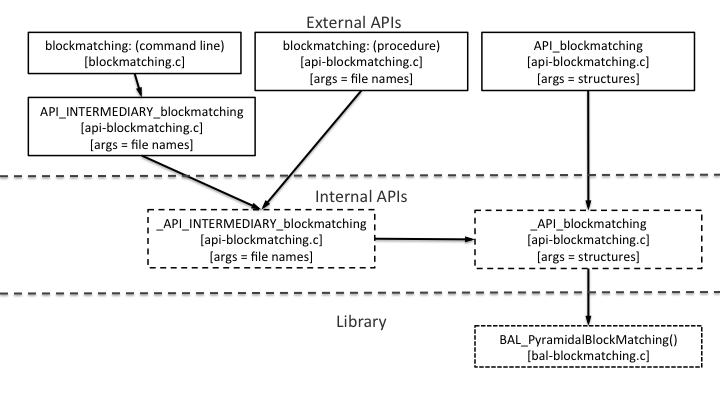
\includegraphics[width=0.8\linewidth]{figures/api-blockmatching.png}
\end{center}
\caption{\label{fig:api:blockmatching} Organization of the blockmatching related APIs.}
\end{figure}
 

\part{Examples of use}

\chapter{Command Line Interfaces}

\section{\pointmatching}
\label{sec:example:pointmatching}

We exemplify here the use of \pointmatching to generate a vector field with two pairings $\{ 
(35,35,0) \rightarrow (60,40,0),
(65,60,0) \rightarrow (40,65,0) \}$, the first points being in the floating image while the second ones are in the reference image (see figure \ref{fig:exe:pointmatching:1}).

Test images can be generated with the following commands. 
\begin{code}{1}
\% createGrid -dim 100 100 mosaic.mha -type mosaic -spacing 10 10 \\
\% createGrid -dim 100 100 grid.mha -spacing 10 10
copy -norma mosaic.mha mosaic.mha
\end{code}

\begin{figure}[ht]
\begin{center}
\begin{tabular}{cc}
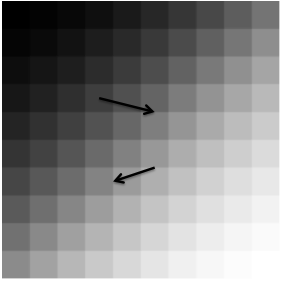
\includegraphics[width=35mm]{use-examples/pointmatching/figures/pairings.png} &
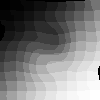
\includegraphics[width=35mm]{use-examples/pointmatching/mosaic-10-10-05.png} \\
&
$(d_p, d_f, \sigma_f) = (10,10,5)$
\end{tabular}
\end{center}
\caption{\label{fig:exe:pointmatching:1} The two pairings superimposed on a mosaic test image, and the resampled image with the deformation computed with $(d_p, d_f, \sigma_f) = (10,10,5)$.}
\end{figure}

The options passed to \pointmatching will be
\begin{code}{1}
-vector-propagation-distance $d_p$
-vector-fading-distance $d_f$
-fluid-sigma $\sigma_f$
\end{code}
where $d_p$, $d_f$, and $\sigma_f$ denotes respectively the propagation distance (of the pairings), the fading distance (of the pairings, after the propagation), and the standard deviation for the regularization (with gaussian interpolation).

Thus, non-linear transformations are computed with different settings for $(d_p, d_f, \sigma_f)$
\begin{code}{1}
\% \pointmatching -flo floating.pts -ref reference.pts -trsf-type vectorfield 
  -template mosaic.mha 
  -vector-propagation-distance $d_p$ 
  -vector-fading-distance $d_f$ 
  -fluid-sigma $\sigma_f$ 
  -res-trsf vectorfield.trsf
\end{code}
and the floating image is resampled thanks to 

\begin{code}{1}
\% \applyTrsf mosaic.mha mosaic-result.mha -trsf vectorfield.trsf -interpolation nearest
\end{code}

\begin{figure}[ht]
\begin{center}
\begin{tabular}{ccc}
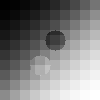
\includegraphics[width=35mm]{use-examples/pointmatching/mosaic-10-00-00.png} &

\includegraphics[width=35mm]{use-examples/pointmatching/mosaic-00-10-00.png} &

\includegraphics[width=35mm]{use-examples/pointmatching/mosaic-00-00-05.png} \\
$(d_p, d_f, \sigma_f) = (10,0,0)$ &
$(d_p, d_f, \sigma_f) = (0,10,0)$ &
$(d_p, d_f, \sigma_f) = (0,0,5)$ 
\end{tabular}
\end{center}
\caption{\label{fig:exe:pointmatching:2} Vector field deformation computation with only one non-null parameter.}
\end{figure}

On figure \ref{fig:exe:pointmatching:2}, it can be seen that deformations calculated with only one non-null parameter among $(d_p, d_f, \sigma_f)$ lead to non-homotopic deformations. Note that using only $\sigma_f$ should act as pure propagation (except at Vorono\"i diagram borders), but due to numerical reasons, the deformation becomes null when gaussian weights are too small.

\begin{figure}[ht]
\begin{center}
\begin{tabular}{ccc}

\includegraphics[width=35mm]{use-examples/pointmatching/mosaic-10-10-00.png} &

\includegraphics[width=35mm]{use-examples/pointmatching/mosaic-10-00-05.png} &

\includegraphics[width=35mm]{use-examples/pointmatching/mosaic-00-10-05.png} \\
$(d_p, d_f, \sigma_f) = (10,10,0)$ &
$(d_p, d_f, \sigma_f) = (10,0,5)$ &
$(d_p, d_f, \sigma_f) = (0,10,5)$ 
\end{tabular}
\end{center}
\caption{\label{fig:exe:pointmatching:3} Vector field deformation computation with only one null parameter.}
\end{figure}

Using two non-null parameters (see figure \ref{fig:exe:pointmatching:3}) allows to get continuous deformations: e.g., $(d_p, d_f, \sigma_f) = (10,0,5)$ and $(d_p, d_f, \sigma_f) = (0,10,5)$. However, deformations may be large at the Vorono\"i diagram borders ($(d_p, d_f, \sigma_f) = (10,0,5)$) or resulting deformations may be quite far away the desired ones ($(d_p, d_f, \sigma_f) = (10,0,5)$). 

Using all the three parameters may yield a deformation close to the expected one (see figure \ref{fig:exe:pointmatching:1}, left). 










\section{\applyTrsf and \blockmatching}
\label{sec:example:applyTrsf:blockmatching}

We exemplified here how to compute a transformation at a lower resolution (also described in section \ref{sec:hand:made:hierarchical:registration}) while still getting a deformed floating image at full resolution. Since the registration computation is done at a lower resolution, it is obviously faster (as it will be by tuning the \option{-pyramid-lowest-level}), but it also requires a little less computer memory. Such an approach can be used to tune parameters for instance.

Input images are of dimensions $481 \times 481$ with a pixel size of 0.5 image (see figure \ref{fig:exe:applyTrsf:blockmatching:1}). They can be non-linearly registered through (registration result can be seen in figure \ref{fig:exe:applyTrsf:blockmatching:1}, middle)
\begin{code}{1}
\% blockmatching -ref ref.mha -flo flo.mha -res res.mha -trsf-type vectorfield -res-trsf vector.trsf -elastic-sigma 2.5 -fluid-sigma 1.0
\end{code}
Options \option{-elastic-sigma 2.5 -fluid-sigma 1.0} have been chosen to enhance deformations.

\begin{figure}[ht]
\begin{center}
\begin{tabular}{ccc}
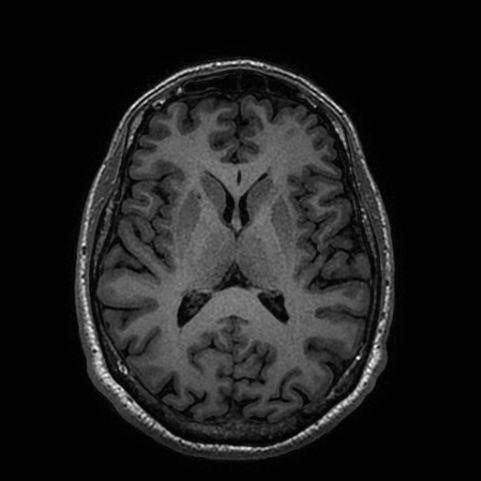
\includegraphics[width=35mm]{use-examples/applyTrsf-blockmatching/ref.png} &
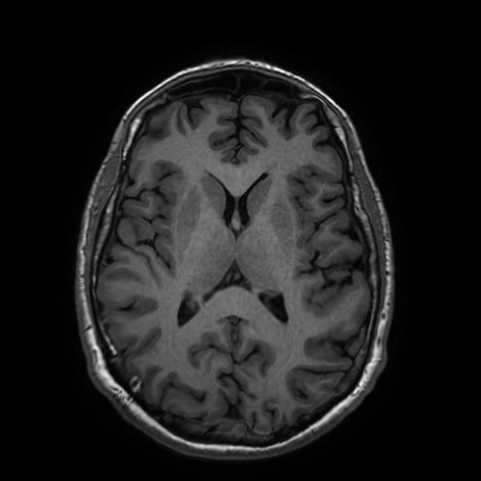
\includegraphics[width=35mm]{use-examples/applyTrsf-blockmatching/res.png} & 
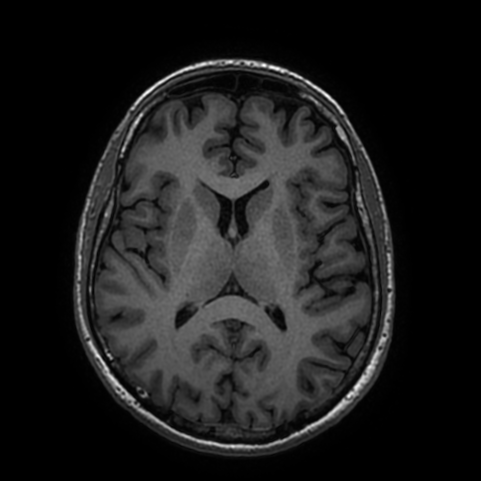
\includegraphics[width=35mm]{use-examples/applyTrsf-blockmatching/flo.png} \\
Reference image &
High resolution result &
Floating image \\
& (deformed floating image) &
\end{tabular}
\end{center}
\caption{\label{fig:exe:applyTrsf:blockmatching:1} Input images for registration. Please notice the smaller ventricles of the floating image. Images dimensions are $481 \times 481$.}
\end{figure}

Input images are downsampled with the following commands (see figure \ref{fig:exe:applyTrsf:blockmatching:2}). Note that, even here the commands are similar, they could have been resampled at different resolutions.
\begin{code}{1}
\% applyTrsf flo.mha lower-flo.mha -iso 2.0 -resize -res-trsf lower-flo.trsf \\
\% applyTrsf ref.mha lower-ref.mha -iso 2.0 -resize -res-trsf lower-ref.trsf
\end{code}
Here images are downsampled to a pixel size of 2.0, yielding images of dimensions $120 \times 120$. These images can be non-linearly registered through  (registration result can be seen in figure \ref{fig:exe:applyTrsf:blockmatching:2}, middle)
\begin{code}{1}
\% blockmatching -ref lower-ref.mha -flo lower-flo.mha -res lower-res.mha -trsf-type vectorfield -res-trsf lower-vector.trsf -elastic-sigma 2.5 -fluid-sigma 1.0
\end{code}

\begin{figure}[ht]
\begin{center}
\begin{tabular}{ccc}
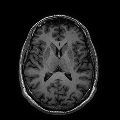
\includegraphics[width=35mm]{use-examples/applyTrsf-blockmatching/lower-ref.png} &
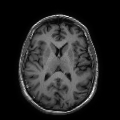
\includegraphics[width=35mm]{use-examples/applyTrsf-blockmatching/lower-res.png} &
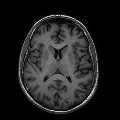
\includegraphics[width=35mm]{use-examples/applyTrsf-blockmatching/lower-flo.png} \\
Reference image &
Low resolution result &
Floating image \\
& (deformed floating image) &
\end{tabular}
\end{center}
\caption{\label{fig:exe:applyTrsf:blockmatching:2} Downsampled images and registration result. Images dimensions are $160 \times 160$.}
\end{figure}

To get the registration result at the original resolution, there are different possibilities.
\begin{enumerate}

\item The low resolution registration result can be upsampled in the same geometry than the reference image. To that end, the downsampling matrix (of the reference image) has first to be inverted. Then, the  low resolution registration result is resampled with this inverted transformation. It can be achieved with
\begin{code}{1}
\% invTrsf lower-ref.trsf inv-lower-ref.trsf \\
\% applyTrsf lower-res.mha resampled-lower-res.mha -trsf inv-lower-ref.trsf -template ref.mha
\end{code}
\begin{figure}[ht]
\begin{center}
\begin{tabular}{ccc}
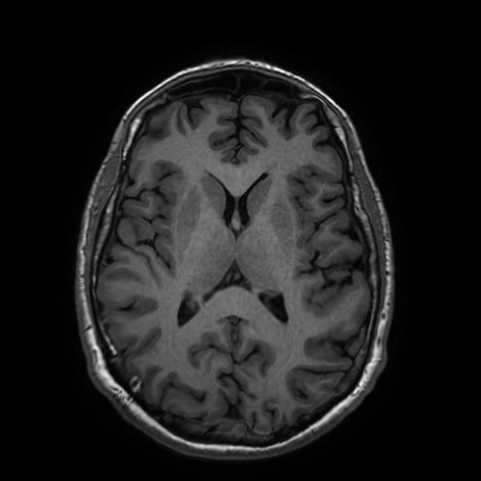
\includegraphics[width=35mm]{use-examples/applyTrsf-blockmatching/res.png} &
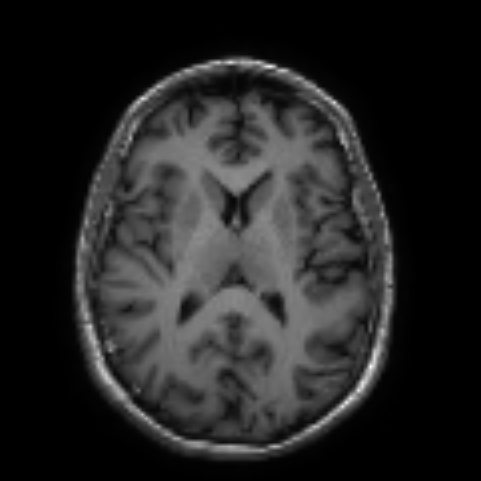
\includegraphics[width=35mm]{use-examples/applyTrsf-blockmatching/resampled-lower-res.png} &
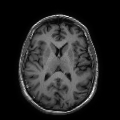
\includegraphics[width=35mm]{use-examples/applyTrsf-blockmatching/lower-res.png} \\
High resolution result &
Upsampled low resolution result &
Low resolution result \\
$481 \times 481$ &
$481 \times 481$ &
$160 \times 160$
\end{tabular}
\end{center}
\caption{\label{fig:exe:applyTrsf:blockmatching:3} Upsampling the low resolution registration result.}
\end{figure}
However, even though the upsampled low resolution registration result is of dimensions $481 \times 481$ with a pixel size of 0.5, the downsampling is visually present (see figure \ref{fig:exe:applyTrsf:blockmatching:3}).

\item A deformation at the high resolution can be computed from the deformation at the low resolution. It comes to compose transformations (see section \ref{sec:hand:made:hierarchical:registration}). The floating image at the high resolution can be then resampled thanks to this transformation. It can be done thanks to
\begin{code}{1}
\% invTrsf lower-ref.trsf inv-lower-ref.trsf \\
\% composeTrsf resampled-lower-vector.trsf -trsfs lower-flo.trsf lower-vector.trsf inv-lower-ref.trsf -template ref.mha \\
\% applyTrsf flo.mha lower-trsf-res.mha -trsf resampled-lower-vector.trsf -template ref.mha
\end{code}
\begin{figure}[ht]
\begin{center}
\begin{tabular}{ccc}
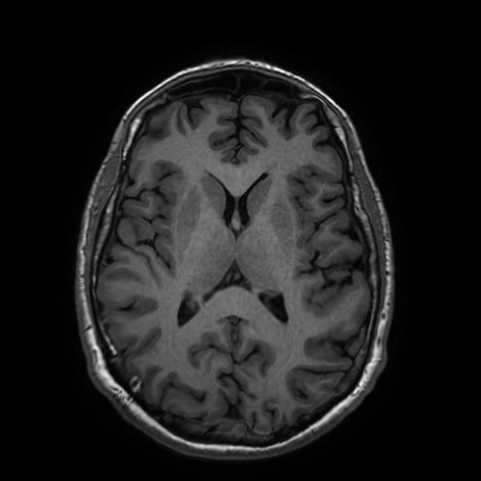
\includegraphics[width=35mm]{use-examples/applyTrsf-blockmatching/res.png} &
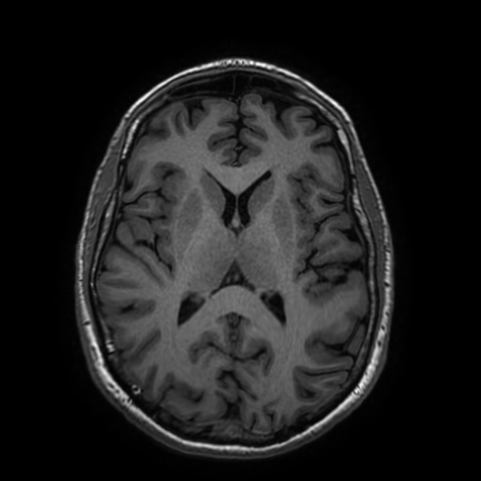
\includegraphics[width=35mm]{use-examples/applyTrsf-blockmatching/lower-trsf-res.png} &
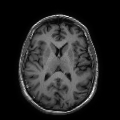
\includegraphics[width=35mm]{use-examples/applyTrsf-blockmatching/lower-res.png} \\
High resolution result &
High resolution result  &
Low resolution result \\
& from low resolution transformation & \\
$481 \times 481$ &
$481 \times 481$ &
$160 \times 160$
\end{tabular}
\end{center}
\caption{\label{fig:exe:applyTrsf:blockmatching:4} Upsampling the low resolution registration result.}
\end{figure}
The result can be see in figure \ref{fig:exe:applyTrsf:blockmatching:4}.

\end{enumerate}




\part{Methodological notes}








\chapter{Frames}
\label{sec:frames}

\section{The digital world ($\mathbb{Z}$)}

Pixels or voxels are defined over $\mathbb{Z}^2$ or $\mathbb{Z}^3$ and have integer coordinates. 


The voxel is a small rectangular cuboid that has a spatial extent. Our conventions are that the voxel coordinates design the center of the voxel. Let $(v_x, v_y, v_z)$ be the voxel size of image $I$, the spatial area of a voxel $M_{\mathbb{R}} = (x,y,z)$ in the real world $\mathbb{R}$ is the cuboid
$[x-v_x/2, x+v_x/2] \times [y-v_y/2, y+v_y/2] \times [z-v_z/2, z+v_z/2]$ (see figure \ref{fig:frame}). 


\begin{figure}[ht]
\begin{center}
 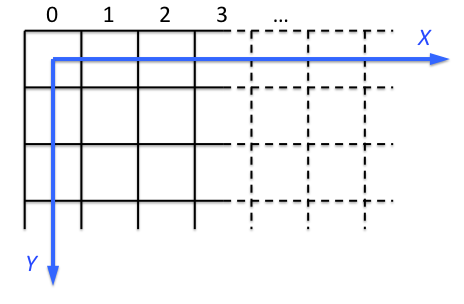
\includegraphics[height=5cm]{figures/fig-frame.png}
\end{center}
\caption{\label{fig:frame}Definition of the  field of view with respect to the  \textit{voxel} one. The origin of the \textit{real} frame is at the center of the upper left pixel/voxel, here the one of coordinate $(0,0,\ldots)$ (C/C++ conventions).}
\end{figure}

Let us consider an image that has a voxel size $v_x$ and a number of voxels of $d_x$ along the $X$ direction. From the C/C++ conventions, the $d_x$ voxels have coordinates in $\mathbb{Z}$ from $0$ to $d_x-1$. The length of the field of view (FOV) is obviously $v_x d_x$ and spans the interval $[v_x * 0 -v_x/2 , v_x*(d_x-1)+v_x/2]
= [-v_x/2, v_x d_x - v_x/2]$ in $\mathbb{R}$.

As a consequence, the center of the field of view in $\mathbb{Z}$ is (here in 3D)
\begin{displaymath}
C_{\mathbb{Z}} = 
\left(
\begin{array}{c}
\frac{(d_{x}-1)}{2} \\
\frac{(d_{y}-1)}{2} \\
\frac{(d_{z}-1)}{2}
\end{array}
\right)
\end{displaymath}

Converting voxel coordinates into real ones can trivially be done by multiplying by the voxel sizes (see section \ref{sec:frame:conversion}). The voxel with zero's coordinates defines then the origin of the \textit{real} frame.

\section{Image: $\mathbb{R} \leftrightarrow \mathbb{Z}$}
\label{sec:frame:conversion}


An image $I$ is defined over the discrete frame $\mathbb{Z}$ and a point $M$ may be defined either by its 'voxel' coordinates $(i,j,k)$, or by 'real' coordinates $(x,y,z)$ that can be deduced from $(i,j,k)$ thanks to the imaging acquisition information.

Conversion from the voxel frame, denoted $\mathbb{Z}$, to the real one, denoted $\mathbb{R}$, is achieved through conversion matrices that are associated with every image $I$.

Without any other specification, there are diagonal matrices with the voxel sizes (or their inverses) along the diagonal. Let $(v_x, v_y, v_z)$ be the voxel size of image $I$, thus a point $M_{\mathbb{R}} = (x,y,z)$ in the real frame $\mathbb{R}$ correspond to the voxel point $M_{\mathbb{Z}} = (i,j,k)$ in the voxel frame $\mathbb{Z}$ with
$$M_{\mathbb{R}} = \mathbf{H}_{I,\mathbb{R} \leftarrow \mathbb{Z}} M_{\mathbb{Z}}
\quad \mbox{ with } \quad
\mathbf{H}_{I,\mathbb{R} \leftarrow \mathbb{Z}} = \left( \begin{array}{cccc}
v_x & . & . & . \\
. & v_y & . & . \\
. & . & v_z & . \\
. & . & . & 1  
\end{array} \right)
$$
Accordingly,
$$M_{\mathbb{Z}} = \mathbf{H}_{I,\mathbb{Z} \leftarrow \mathbb{R}} M_{\mathbb{R}}
\quad \mbox{ with } \quad
\mathbf{H}_{I,\mathbb{Z} \leftarrow \mathbb{R}} = \left( \begin{array}{cccc}
1/v_x & . & . & . \\
. & 1/v_y & . & . \\
. & . & 1/v_z & . \\
. & . & . & 1  
\end{array} \right)
$$
Obviously, we have $\mathbf{H}_{I,\mathbb{Z} \leftarrow \mathbb{R}} = \mathbf{H}^{-1}_{I,\mathbb{R} \leftarrow \mathbb{Z}}$. Note that we use homogeneous coordinates (see section \ref{sec:homogeneous}) to define these matrices.


\begin{attention}
With such a default convention, the frame origins in both the real and the voxel frames superimpose. However, the frame origin in the real frame is not the upper left corner of the field of view (see figure \ref{fig:frame}).
\end{attention}

Note that the matrix $\mathbf{H}$ can be any linear matrix. E.g. they can be reorientation matrices that allows to map the voxel array in standard radiology conventions \footnote{Nifti and Inrimage image formats can embed such rigid transformations (the so-called qform matrices in Nifti format). However, such information can be lost when converting to other formats.}.






%%%%%%%%%%%%%%%%%%%%%%%%%%%%%%%%%%%%%%%
%
% transformations
%
%%%%%%%%%%%%%%%%%%%%%%%%%%%%%%%%%%%%%%%





\chapter{Transformations}


\section{Definitions}

\subsection{Linear transformations}

Classically, linear transformations (i.e. translations, rigid transformations, affine transformations, etc.) are expressed as combinations of a $3 \times 3$ matrix (representing the vectorial part of the transformation) $\mathbf{A}$ and a 3D vector $\mathbf{t}$ (representing the translation). Thus, the transformed point $M'$ of $M$ by the transformation $T=(\mathbf{A},\mathbf{t})$ is expressed by
\begin{displaymath}
M' = T(M) = \mathbf{A} M + \mathbf{t}
\end{displaymath}

Note that linear transformations are mainly expressed in homogeneous coordinates all along this document (see section \ref{sec:homogeneous:linear}), thus we will use the somewhat abusive notation
\begin{displaymath}
M' = \mathbf{T} M 
\end{displaymath}
where $\mathbf{T}$ is a $4 \times 4$ matrix.

\subsection{Vector fields}

Vector fields are used to encode non-linear transformations. For a transformation $T$, the vector $\mathbf{v}(M)$ at point $M$ is the displacement of the point $M$, meaning that 
\begin{displaymath}
M' = T(M) = M + \mathbf{v}(M)
\end{displaymath}







\section{Homogeneous coordinates}
\label{sec:homogeneous}

4D homogeneous coordinates are implicitly used. However, there are some  with transformations expressed as vector fields. 

\subsection{Linear transformations}
\label{sec:homogeneous:linear}

It is more convenient to express the linear transformations as $4 \times 4$ matrices embedding the translation, so combinations of linear transformations can be expressed by multiplications of matrices. Such a $4 \times 4$ matrix $\mathbf{T}$ is designed by
\begin{displaymath}
\mathbf{T} =
\left(
\begin{array}{ccc|c}
& & & \\
& \mathbf{A} & & \mathbf{t} \\
& & & \\ \hline
0 & 0 & 0 & 1
\end{array}
\right)
\end{displaymath}

A point $M$ has then implicitly 4 coordinates, the first three ones being the spatial coordinates $(x,y,z)$ and the last one being 1. We have thus 
\begin{displaymath}
M'
= T(M)
=
\left(
\begin{array}{l}
x' \\ y' \\ z' \\ 1
\end{array}
\right)
= \mathbf{T} M
= 
\left(
\begin{array}{ccc|c}
& & & \\
& \mathbf{A} & & \mathbf{t} \\
& & & \\ \hline
0 & 0 & 0 & 1
\end{array}
\right)
\left(
\begin{array}{l}
x \\ y \\ z \\ 1
\end{array}
\right)
\end{displaymath}


\subsection{Vector fields}

The transformation with a vector field is encoded by 
\begin{displaymath}
M' = M + \mathbf{v}(M)
\end{displaymath}
When composing (at left) with a linear transformation, we have
\begin{eqnarray}
M'' & = & \mathbf{A} M' + \mathbf{t} \nonumber \\
& = & \mathbf{A} M + \mathbf{A} \mathbf{v}(M) + \mathbf{t}
\label{eq:composition:linear:vector}
\end{eqnarray}

If homogeneous coordinates are used, it comes
\begin{eqnarray*}
M'' & = & \mathbf{T} M' 
\left( = \mathbf{A} M' + \mathbf{t} \right) \\
& = & \mathbf{T} M + \mathbf{T} \mathbf{v}(M) 
\end{eqnarray*}
From equation \ref{eq:composition:linear:vector}, it comes that 
\begin{displaymath}
\mathbf{T} \mathbf{v}(M) = \mathbf{A} \mathbf{v}(M)
\end{displaymath}
This is compatible with homogeneous coordinates if the fourth coordinate of $\mathbf{v}$ is $0$, indeed
\begin{displaymath}
\mathbf{T} \mathbf{v}
= 
\left(
\begin{array}{ccc|c}
& & & \\
& \mathbf{A} & & \mathbf{t} \\
& & & \\ \hline
0 & 0 & 0 & 1
\end{array}
\right)
\left(
\begin{array}{c}
\mathbf{v}_x \\ \mathbf{v}_y \\ \mathbf{v}_z \\ 0
\end{array}
\right)
= 
\left(
\begin{array}{c}
\mathbf{A} \mathbf{v} \\ \hline
0
\end{array}
\right)
\end{displaymath}













\section{'voxel' versus 'real' definitions}

%definitions for discrete images; $\mathbb{R} \leftrightarrow \mathbb{Z}$ conversion}

Recall that an image $I$ is defined over the discrete frame $\mathbb{Z}$. Thus a point $M$ of $I$ can be expressed either in the discrete frame in voxel coordinates (and will be denoted $M_{\mathbb{Z}}$) or in real coordinates (and will be denoted $M_{\mathbb{R}}$). Conversion matrices (see section \ref{sec:frame:conversion}) allow to go from the voxel frame to the real one, and conversely.

A transformation $T_{flo \leftarrow ref}$ from an image $I_{ref}$ towards an image $I_{flo}$ can be then either defined in the voxel frame or in the real one. These transformations are denoted respectively $T_{flo \leftarrow ref,\mathbb{Z}}$ and $T_{flo \leftarrow ref,\mathbb{R}}$:
\begin{displaymath}
\begin{array}{ll}
T_{flo \leftarrow ref,\mathbb{Z}}: &
I_{ref} \rightarrow I_{flo}\\
& M_{ref,\mathbb{Z}} \mapsto M_{flo,\mathbb{Z}}
\end{array}
\end{displaymath}
and
\begin{displaymath}
\begin{array}{ll}
T_{flo \leftarrow ref,\mathbb{R}}: &
I_{ref} \rightarrow I_{flo}\\
& M_{ref,\mathbb{R}} \mapsto M_{flo,\mathbb{R}}
\end{array}
\end{displaymath}

We have then 
\begin{eqnarray*}
M_{flo,\mathbb{Z}} & = & 
T_{flo \leftarrow ref,\mathbb{Z}}(M_{ref,\mathbb{Z}}) \\
M_{flo,\mathbb{R}} & = & 
T_{flo \leftarrow ref,\mathbb{R}}(M_{ref,\mathbb{R}})
\end{eqnarray*}

Transformations in 'voxel' coordinates are required for image resampling, while transformations in 'real' coordinates may be necessary when dealing when some transformation classes (e.g. rigid) or to compute some measurements (e.g. mean displacements) in world units. Thus, conversion of these transformations from the voxel world to the real one, using the image conversion matrices (see section \ref{sec:frame:conversion}), has to be made explicit.

\subsection{Linear transformations}

Linear transformations can be expressed by $4x4$ matrices in homogeneous coordinates (see section \ref{sec:homogeneous:linear}), thus we have 
\begin{eqnarray*}
M_{flo,\mathbb{Z}} & = & 
T_{flo \leftarrow ref,\mathbb{Z}} M_{ref,\mathbb{Z}}  \\
M_{flo,\mathbb{R}} & = & 
T_{flo \leftarrow ref,\mathbb{R}} M_{ref,\mathbb{R}}
\end{eqnarray*}

To convert the transformations from the voxel world to the real one (and conversely), we apply the composition rules that are here simply matrices multiplication:
$$
\mathbf{T}_{flo \leftarrow ref, \mathbb{Z}} 
=
\mathbf{H}_{flo,\mathbb{Z} \leftarrow \mathbb{R}} \circ
\mathbf{T}_{flo \leftarrow ref, \mathbb{R}} \circ
\mathbf{H}_{ref,\mathbb{R} \leftarrow \mathbb{Z}}
$$
and
$$
\mathbf{T}_{flo \leftarrow ref, \mathbb{R}} 
=
\mathbf{H}_{flo,\mathbb{R} \leftarrow \mathbb{Z}} \circ
\mathbf{T}_{flo \leftarrow ref, \mathbb{Z}} \circ
\mathbf{H}_{ref,\mathbb{Z} \leftarrow \mathbb{R}}
$$


\subsection{Vector fields}

The difficulty comes from the fact that the non-linear transformation is encoded by a displacement/vector field that is defined over a discrete lattice (i.e. an image). We have then
\begin{eqnarray*}
M_{flo,\mathbb{Z}} & = & 
T_{flo \leftarrow ref,\mathbb{Z}}(M_{ref,\mathbb{Z}}) \\
& = &
M_{ref,\mathbb{Z}} + 
\mathbf{v}_{flo \leftarrow ref, \mathbb{Z}}(M_{ref, \mathbb{Z}}) \\
M_{flo,\mathbb{R}} & = & 
T_{flo \leftarrow ref,\mathbb{R}}(M_{ref,\mathbb{R}}) \\
& = &
M_{ref,\mathbb{R}} + 
\mathbf{v}_{flo \leftarrow ref, \mathbb{R}}(M_{ref, \mathbb{Z}}) \\
& = &
M_{ref,\mathbb{R}} + 
\mathbf{v}_{flo \leftarrow ref, \mathbb{R}}(\mathbf{H}_{ref, \mathbb{Z} \leftarrow \mathbb{R}}  M_{ref, \mathbb{R}})
\end{eqnarray*}
where $\mathbf{H}_{ref, \mathbb{Z} \leftarrow \mathbb{R}}$ denotes the conversion matrix from the real world $\mathbb{R}$ to the discrete world $\mathbb{Z}$ for image $I_{ref}$.

The vector field $\mathbf{v}$ indicates the displacement at every point. For a transformation from image $I_{ref}$ to image $I_{flo}$, this vector is defined on the same frame than $I_{ref}$. Thus the vector in \textit{real} coordinates $\mathbf{v}_{flo \leftarrow ref, \mathbb{R}}$ at $M_{\mathbb{R}}$ gives the displacement of the point $M_{\mathbb{R}}$.

However, since $\mathbf{v}_{flo \leftarrow ref}$ is defined over a discrete lattice, the vector image stores the vectors $\mathbf{v}_{\mathbb{R}}(M_{\mathbb{Z}})$, thus $\mathbf{v}_{\mathbb{R}}$ at $M_{\mathbb{R}}$ is $\mathbf{v}_{\mathbb{R}}( \mathbf{H}_{\mathbb{Z} \leftarrow \mathbb{R}} M_{\mathbb{R}} )$.


\subsubsection{Vector fields: $\mathbb{R} \rightarrow \mathbb{Z}$}




The transformation $\mathbf{T}_{flo \leftarrow ref, \mathbb{R}}$ from image $I_{ref}$ to image $I_{flo}$ is defined by the vector field $\mathbf{v}_{flo \leftarrow ref,\mathbb{R}}$
\begin{eqnarray*}
M_{flo,\mathbb{R}} & = & 
\mathbf{T}(M_{ref,\mathbb{R}}) = M_{ref,\mathbb{R}} + \mathbf{v}_{flo \leftarrow ref,\mathbb{R}}( \mathbf{H}_{ref, \mathbb{Z} \leftarrow \mathbb{R}} M_{ref,\mathbb{R}} )\\
& = & 
\mathbf{T}(M_{ref,\mathbb{R}}) = M_{ref,\mathbb{R}} + \mathbf{v}_{flo \leftarrow ref,\mathbb{R}}(M_{ref,\mathbb{Z}} )
\end{eqnarray*}

When expressing this formula in the discrete lattice, it comes
\begin{displaymath}
\mathbf{H}_{flo, \mathbb{R} \leftarrow \mathbb{Z}} M_{flo,\mathbb{Z}}
=
\mathbf{H}_{ref, \mathbb{R} \leftarrow \mathbb{Z}} M_{ref,\mathbb{Z}}
+ \mathbf{v}_{flo \leftarrow ref,\mathbb{R}}( M_{ref,\mathbb{Z}} )
\end{displaymath}
\begin{displaymath}
M_{flo,\mathbb{Z}} 
=
\mathbf{H}^{-1}_{flo, \mathbb{R} \leftarrow \mathbb{Z}}
\circ \mathbf{H}_{ref, \mathbb{R} \leftarrow \mathbb{Z}} 
M_{ref,\mathbb{Z}}
+ \mathbf{H}^{-1}_{flo, \mathbb{R} \leftarrow \mathbb{Z}}
\circ \mathbf{v}_{flo \leftarrow ref,\mathbb{R}}( M_{ref,\mathbb{Z}} )
\end{displaymath}


The displacement in \textit{voxel} coordinates $\mathbf{v}_{flo \leftarrow ref,\mathbb{Z}}$ (associated to $\mathbf{T}_{flo \leftarrow ref,\mathbb{Z}}$) is then defined by
\begin{eqnarray*}
\lefteqn{\mathbf{v}_{flo \leftarrow ref,\mathbb{Z}}( M_{ref,\mathbb{Z}} )
 =  M_{flo,\mathbb{Z}} - M_{ref,\mathbb{Z}}} \\
& = & 
\left( \mathbf{H}^{-1}_{flo, \mathbb{R} \leftarrow \mathbb{Z}}
 \circ \mathbf{H}_{ref, \mathbb{R} \leftarrow \mathbb{Z}} - \mathbf{Id} \right)
 M_{ref,\mathbb{Z}}
 + \mathbf{H}^{-1}_{flo, \mathbb{R} \leftarrow \mathbb{Z}}
 \circ \mathbf{v}_{flo \leftarrow ref,\mathbb{R}}( M_{ref,\mathbb{Z}} ) \\
 & = & 
\left( \mathbf{H}_{flo, \mathbb{Z} \leftarrow \mathbb{R}}
 \circ \mathbf{H}_{ref, \mathbb{R} \leftarrow \mathbb{Z}} - \mathbf{Id} \right)
 M_{ref,\mathbb{Z}}
 + \mathbf{H}_{flo, \mathbb{Z} \leftarrow \mathbb{R}}
 \circ \mathbf{v}_{flo \leftarrow ref,\mathbb{R}}( M_{ref,\mathbb{Z}} ) \\
\end{eqnarray*}
(where $\mathbf{Id}$ denotes the identity matrix) and may be different from a simple scaling of the vector field defined in \textit{real} coordinates.

\subsubsection{Vector fields: $\mathbb{Z} \rightarrow \mathbb{R}$}

We have 
\begin{displaymath}
M_{flo,\mathbb{Z}} = M_{ref,\mathbb{Z}} 
+ \mathbf{v}_{flo \leftarrow ref,\mathbb{Z}}( M_{ref,\mathbb{Z}} )
\end{displaymath}

When expressing this formula in the real world, it comes
\begin{displaymath}
\mathbf{H}_{flo, \mathbb{Z} \leftarrow \mathbb{R}} 
M_{flo,\mathbb{R}}
=
\mathbf{H}_{ref, \mathbb{Z} \leftarrow \mathbb{R}} 
M_{ref,\mathbb{R}}
+ \mathbf{v}_{flo \leftarrow ref,\mathbb{Z}}( M_{ref,\mathbb{Z}} ) \\
\end{displaymath}
\begin{displaymath}
M_{flo,\mathbb{R}}
=
\mathbf{H}^{-1}_{flo, \mathbb{Z} \leftarrow \mathbb{R}}
\circ 
\mathbf{H}_{ref, \mathbb{Z} \leftarrow \mathbb{R}}
M_{ref,\mathbb{R}}
+ 
\mathbf{H}^{-1}_{flo, \mathbb{Z} \leftarrow \mathbb{R}}
\circ \mathbf{v}_{flo \leftarrow ref,\mathbb{Z}}( M_{ref,\mathbb{Z}} )
\end{displaymath}

The displacement in \textit{real} coordinates $\mathbf{v}_{flo \leftarrow ref,\mathbb{R}}$ is then defined by
\begin{eqnarray*}
\lefteqn{
\mathbf{v}_{flo \leftarrow ref,\mathbb{R}}( M_{ref,\mathbb{Z}} )
= M_{flo,\mathbb{R}} - M_{ref,\mathbb{R}}} \\
& = & 
\left(
\mathbf{H}^{-1}_{flo, \mathbb{Z} \leftarrow \mathbb{R}}
\circ 
\mathbf{H}_{ref, \mathbb{Z} \leftarrow \mathbb{R}}
- \mathbf{Id} \right) M_{ref,\mathbb{R}}
+ 
\mathbf{H}^{-1}_{flo, \mathbb{Z} \leftarrow \mathbb{R}}
\circ \mathbf{v}_{flo \leftarrow ref,\mathbb{Z}}( M_{ref,\mathbb{Z}} ) \\
& = & 
\left(
\mathbf{H}^{-1}_{flo, \mathbb{Z} \leftarrow \mathbb{R}}
\circ 
\mathbf{H}_{ref, \mathbb{Z} \leftarrow \mathbb{R}}
- \mathbf{Id} \right) 
\mathbf{H}_{ref, \mathbb{R} \leftarrow \mathbb{Z}}
M_{ref,\mathbb{Z}}
+ 
\mathbf{H}_{flo, \mathbb{R} \leftarrow \mathbb{Z}}
\circ \mathbf{v}_{flo \leftarrow ref,\mathbb{Z}}( M_{ref,\mathbb{Z}} ) \\
& = & 
\left(
\mathbf{H}_{flo, \mathbb{R} \leftarrow \mathbb{Z}}
-
\mathbf{H}_{ref, \mathbb{R} \leftarrow \mathbb{Z}}
\right)
M_{ref,\mathbb{Z}}
+ 
\mathbf{H}_{flo, \mathbb{R} \leftarrow \mathbb{Z}}
\circ \mathbf{v}_{flo \leftarrow ref,\mathbb{Z}}( M_{ref,\mathbb{Z}} ) \\
\end{eqnarray*}





\section{Transformations: linear $\rightarrow$ vector field}

$\mathbf{T}_{flo \leftarrow ref, \mathbb{R}}$ is a linear transformation in real space. We have then
\begin{displaymath}
M_{flo, \mathbb{R}} = 
\mathbf{T}_{flo \leftarrow ref, \mathbb{R}}
M_{ref, \mathbb{R}}
\end{displaymath}
For vector fields, the transformation is expressed by
\begin{displaymath}
M_{flo, \mathbb{R}} = 
M_{ref, \mathbb{R}} 
+ \mathbf{v}_{flo \leftarrow ref, \mathbb{R}}(M_{ref, \mathbb{Z}})
\end{displaymath}
We have then
\begin{eqnarray*}
\mathbf{v}_{flo \leftarrow ref, \mathbb{R}}(M_{ref, \mathbb{Z}}) & = & 
M_{flo, \mathbb{R}} - M_{ref, \mathbb{R}} \\
& = &
\mathbf{T}_{flo \leftarrow ref, \mathbb{R}}
M_{ref, \mathbb{R}} - M_{ref, \mathbb{R}} \\
& = &
\left( \mathbf{T}_{flo \leftarrow ref, \mathbb{R}} - \mathbf{Id} \right) \circ
\mathbf{H}_{ref, \mathbb{R} \leftarrow \mathbb{Z}} M_{ref, \mathbb{Z}} \\
& = &
\left( \mathbf{H}_{flo,\mathbb{R} \leftarrow \mathbb{Z}} \circ
\mathbf{T}_{flo \leftarrow ref, \mathbb{Z}} \circ
\mathbf{H}_{ref,\mathbb{Z} \leftarrow \mathbb{R}} - \mathbf{Id} \right) \circ
\mathbf{H}_{ref, \mathbb{R} \leftarrow \mathbb{Z}} M_{ref, \mathbb{Z}} \\
\end{eqnarray*}

Remarks:
\begin{itemize}

\item Estimating the vector field in real/world units $\mathbf{v}_{flo \leftarrow ref, \mathbb{R}}$ from a linear transformation in real/world units $\mathbf{T}_{flo \leftarrow ref, \mathbb{Z}}$ is done with 
\begin{displaymath}
\left( \mathbf{T}_{flo \leftarrow ref, \mathbb{R}} - \mathbf{Id} \right) \circ
\mathbf{H}_{ref, \mathbb{R} \leftarrow \mathbb{Z}} M_{ref, \mathbb{Z}}
\end{displaymath}
Note that the voxel-to-world transformation for the reference image/frame $\mathbf{H}_{ref, \mathbb{R} \leftarrow \mathbb{Z}}$ is also embedded in the non-linear transformation $\mathbf{v}_{flo \leftarrow ref, \mathbb{R}}$.

\item Estimating the vector field in real/world units $\mathbf{v}_{flo \leftarrow ref, \mathbb{R}}$ from a linear transformation in voxel units $\mathbf{T}_{flo \leftarrow ref, \mathbb{Z}}$ 
\begin{eqnarray*}
\lefteqn{\mathbf{v}_{flo \leftarrow ref, \mathbb{R}}(M_{ref, \mathbb{Z}}) = } \\
& &
\left( \mathbf{H}_{flo,\mathbb{R} \leftarrow \mathbb{Z}} \circ
\mathbf{T}_{flo \leftarrow ref, \mathbb{Z}} \circ
\mathbf{H}_{ref,\mathbb{Z} \leftarrow \mathbb{R}} - \mathbf{Id} \right) \circ
\mathbf{H}_{ref, \mathbb{R} \leftarrow \mathbb{Z}} M_{ref, \mathbb{Z}}
\end{eqnarray*}
requires to have the voxel-to-world transformation for the floating image/frame $\mathbf{H}_{flo,\mathbb{R} \leftarrow \mathbb{Z}}$ at hand.

\item When $\mathbf{T}_{flo \leftarrow ref, \mathbb{R}}$ is a pure translation $\mathbf{t}_{\mathbb{R}}$, meaning that 
$M_{flo, \mathbb{R}} = 
\mathbf{Id} M_{ref, \mathbb{R}} + \mathbf{t}_{\mathbb{R}}$, we have then
\begin{displaymath}
\mathbf{v}_{flo \leftarrow ref, \mathbb{R}}(M_{ref, \mathbb{Z}}) = \mathbf{t}_{\mathbb{R}}
\end{displaymath}

\end{itemize}










\section{Transformation composition}

We simply use the composition rules to  transformation composition.
\begin{displaymath}
\mathbf{T}_{K \leftarrow I, \mathbb{R}}
= 
\mathbf{T}_{K \leftarrow J, \mathbb{R}}
\circ
\mathbf{T}_{J \leftarrow I, \mathbb{R}}
\end{displaymath}
and
\begin{displaymath}
\mathbf{T}_{K \leftarrow I, \mathbb{Z}}
= 
\mathbf{T}_{K \leftarrow J, \mathbb{Z}}
\circ
\mathbf{T}_{J \leftarrow I, \mathbb{Z}}
\end{displaymath}



\subsection{Linear $\circ$ linear}

The composition is quite trivial, since it only uses matrices multiplication.



\subsection{Linear $\circ$ vector field in $\mathbb{R}$ }

\begin{eqnarray*}
M_{J, \mathbb{R}} & = &
M_{I, \mathbb{R}} 
+ \mathbf{v}_{J \leftarrow I, \mathbb{R}}
(\mathbf{H}_{I, \mathbb{Z} \leftarrow \mathbb{R}}  M_{I, \mathbb{R}}) \\
& = & 
\mathbf{H}_{I, \mathbb{R} \leftarrow \mathbb{Z}} M_{I, \mathbb{Z}}
+ \mathbf{v}_{J \leftarrow I, \mathbb{R}}(M_{I, \mathbb{Z}}) \\
M_{K, \mathbb{R}} & = &
 \mathbf{T}_{K \leftarrow J, \mathbb{R}} M_{J, \mathbb{R}} \\
& = &
\mathbf{T}_{K \leftarrow J, \mathbb{R}} 
\mathbf{H}_{I, \mathbb{R} \leftarrow \mathbb{Z}} 
M_{I, \mathbb{Z}} 
+ \mathbf{T}_{K \leftarrow J, \mathbb{R}} 
\mathbf{v}_{J \leftarrow I, \mathbb{R}}(M_{I, \mathbb{Z}})
\end{eqnarray*}

\begin{eqnarray*}
\mathbf{v}_{K \leftarrow I, \mathbb{R}}(M_{I, \mathbb{Z}})
& = &
M_{K, \mathbb{R}} - M_{I, \mathbb{R}} \\
& = &
\left( \mathbf{T}_{K \leftarrow J, \mathbb{R}} - \mathbf{Id} \right)
\circ 
\mathbf{H}_{I, \mathbb{R} \leftarrow \mathbb{Z}} 
M_{I, \mathbb{Z}} 
+ \mathbf{T}_{K \leftarrow J, \mathbb{R}} 
\mathbf{v}_{J \leftarrow I, \mathbb{R}}(M_{I, \mathbb{Z}})
\end{eqnarray*}



\subsection{Linear $\circ$ vector field in $\mathbb{Z}$ }

\begin{eqnarray*}
M_{J, \mathbb{Z}} & = &
M_{I, \mathbb{Z}} 
+ \mathbf{v}_{J \leftarrow I, \mathbb{Z}}(M_{I, \mathbb{Z}}) \\
M_{K, \mathbb{Z}} & = &
 \mathbf{T}_{K \leftarrow J, \mathbb{Z}} M_{J, \mathbb{Z}} \\
& = &
\mathbf{T}_{K \leftarrow J, \mathbb{Z}} 
M_{I, \mathbb{Z}} 
+ \mathbf{T}_{K \leftarrow J, \mathbb{Z}} 
\mathbf{v}_{J \leftarrow I, \mathbb{Z}}(M_{I, \mathbb{Z}})
\end{eqnarray*}

\begin{eqnarray*}
\mathbf{v}_{K \leftarrow I, \mathbb{Z}}(M_{I, \mathbb{Z}})
& = &
M_{K, \mathbb{Z}} - M_{I, \mathbb{Z}} \\
& = &
\left( \mathbf{T}_{K \leftarrow J, \mathbb{Z}} - \mathbf{Id} \right)
M_{I, \mathbb{Z}} 
+ \mathbf{T}_{K \leftarrow J, \mathbb{Z}} 
\mathbf{v}_{J \leftarrow I, \mathbb{Z}}(M_{I, \mathbb{Z}})
\end{eqnarray*}





\subsection{Vector field $\circ$ linear in $\mathbb{R}$ }

\begin{eqnarray*}
M_{J, \mathbb{R}} & = &  
\mathbf{T}_{J \leftarrow I, \mathbb{R}} M_{I, \mathbb{R}}  \\
M_{K, \mathbb{R}} & = &
M_{J, \mathbb{R}} 
+ \mathbf{v}_{K \leftarrow J, \mathbb{R}}(\mathbf{H}_{J, \mathbb{Z} \leftarrow \mathbb{R}}  M_{J, \mathbb{R}}) \\
& = &
\mathbf{T}_{J \leftarrow I, \mathbb{R}} M_{I, \mathbb{R}}
+ \mathbf{v}_{K \leftarrow J, \mathbb{R}}(\mathbf{H}_{J, \mathbb{Z} \leftarrow \mathbb{R}}  \mathbf{T}_{J \leftarrow I, \mathbb{R}} M_{I, \mathbb{R}} )
\end{eqnarray*}

\begin{eqnarray*}
\mathbf{v}_{K \leftarrow I, \mathbb{R}}(M_{I, \mathbb{Z}})
& = &
M_{K, \mathbb{R}} - M_{I, \mathbb{R}} \\
& = &
\left( \mathbf{T}_{J \leftarrow I, \mathbb{R}} - \mathbf{Id} \right)
\circ 
\mathbf{H}_{I, \mathbb{R} \leftarrow \mathbb{Z}} 
M_{I, \mathbb{Z}}  \\
& & {}
+ 
\mathbf{v}_{K \leftarrow J, \mathbb{R}}
(\mathbf{H}_{J, \mathbb{Z} \leftarrow \mathbb{R}}
\mathbf{T}_{J \leftarrow I, \mathbb{R}} 
\mathbf{H}_{I, \mathbb{R} \leftarrow \mathbb{Z}}
M_{I, \mathbb{Z}} )
\end{eqnarray*}



\subsection{Vector field $\circ$ linear in $\mathbb{Z}$ }

\begin{eqnarray*}
M_{J, \mathbb{Z}} &  =  &
\mathbf{T}_{J \leftarrow I, \mathbb{Z}} M_{I, \mathbb{Z}} \\
M_{K, \mathbb{Z}} & = &
M_{J, \mathbb{Z}} 
+ \mathbf{v}_{K \leftarrow J, \mathbb{Z}}(M_{J, \mathbb{Z}}) \\
& = &
\mathbf{T}_{J \leftarrow I, \mathbb{Z}} M_{I, \mathbb{Z}} 
+ \mathbf{v}_{K \leftarrow J, \mathbb{Z}}(\mathbf{T}_{J \leftarrow I, \mathbb{Z}} M_{I, \mathbb{Z}} )
\end{eqnarray*}

\begin{eqnarray*}
\mathbf{v}_{K \leftarrow I, \mathbb{Z}}(M_{I, \mathbb{Z}})
& = &
M_{K, \mathbb{Z}} - M_{I, \mathbb{Z}} \\
& = &
\left( \mathbf{T}_{J \leftarrow I, \mathbb{Z}} - \mathbf{Id} \right)
M_{I, \mathbb{Z}}
+ \mathbf{v}_{K \leftarrow J, \mathbb{Z}}
( \mathbf{T}_{J \leftarrow I, \mathbb{Z}} M_{I, \mathbb{Z}} )
\end{eqnarray*}


\subsection{Vector field $\circ$ vector field in $\mathbb{R}$ }

\begin{eqnarray*}
M_{J, \mathbb{R}} & =  &
M_{I, \mathbb{R}} 
+ \mathbf{v}_{J \leftarrow I, \mathbb{R}}(\mathbf{H}_{I, \mathbb{Z} \leftarrow \mathbb{R}}  M_{I, \mathbb{R}}) \\
& = &
\mathbf{H}_{I, \mathbb{R} \leftarrow \mathbb{Z}} M_{I, \mathbb{Z}}
+ \mathbf{v}_{J \leftarrow I, \mathbb{R}}(M_{I, \mathbb{Z}}) \\
M_{K, \mathbb{R}} & = &
M_{J, \mathbb{R}} 
+ \mathbf{v}_{K \leftarrow J, \mathbb{R}}(\mathbf{H}_{J, \mathbb{Z} \leftarrow \mathbb{R}}  M_{J, \mathbb{R}}) \\
& = &
M_{I, \mathbb{R}}
+ \mathbf{v}_{J \leftarrow I, \mathbb{R}}(M_{I, \mathbb{Z}}) \\
& & {}
+ \mathbf{v}_{K\leftarrow J, \mathbb{R}}\left(
\mathbf{H}_{J, \mathbb{Z} \leftarrow \mathbb{R}} 
\left( 
\mathbf{H}_{I, \mathbb{R} \leftarrow \mathbb{Z}} M_{I, \mathbb{Z}}
+ 
\mathbf{v}_{J \leftarrow I, \mathbb{R}}(M_{I, \mathbb{Z}}
\right)
\right)
\end{eqnarray*}


\begin{eqnarray*}
\mathbf{v}_{K \leftarrow I, \mathbb{R}}(M_{I, \mathbb{Z}})
& = &
M_{K, \mathbb{R}} - M_{I, \mathbb{R}} \\
& = &
\mathbf{v}_{J \leftarrow I, \mathbb{R}}(M_{I, \mathbb{Z}}) \\
& & {}
+ \mathbf{v}_{K \leftarrow J, \mathbb{R}}
\left(
\mathbf{H}_{J, \mathbb{Z} \leftarrow \mathbb{R}} 
\left( 
\mathbf{H}_{I, \mathbb{R} \leftarrow \mathbb{Z}} M_{I, \mathbb{Z}}
+ 
\mathbf{v}_{J \leftarrow I, \mathbb{R}}(M_{I, \mathbb{Z}}
\right)
\right) \\
& = &
\mathbf{v}_{J \leftarrow I, \mathbb{R}}(M_{I, \mathbb{Z}}) \\
& & {}
+ \mathbf{v}_{K \leftarrow J, \mathbb{R}}
\left(
\mathbf{H}_{J, \mathbb{Z} \leftarrow \mathbb{R}} 
\circ
\mathbf{H}_{I, \mathbb{R} \leftarrow \mathbb{Z}} M_{I, \mathbb{Z}}
+ 
\mathbf{H}_{J, \mathbb{Z} \leftarrow \mathbb{R}} 
\circ \mathbf{v}_{J \leftarrow I, \mathbb{R}}(M_{I, \mathbb{Z}})
\right)
\end{eqnarray*}





\subsection{Vector field $\circ$ vector field in $\mathbb{Z}$ }


\begin{eqnarray*}
M_{J, \mathbb{Z}} & =  &
M_{I, \mathbb{Z}} 
+ \mathbf{v}_{J \leftarrow I, \mathbb{Z}}( M_{I, \mathbb{Z}}) \\
M_{K, \mathbb{Z}} & = &
M_{J, \mathbb{Z}} 
+ \mathbf{v}_{K \leftarrow J, \mathbb{Z}}(M_{J, \mathbb{Z}}) \\
& = &
M_{I, \mathbb{Z}}
+ \mathbf{v}_{J \leftarrow I, \mathbb{Z}}(M_{I, \mathbb{Z}}) 
+ \mathbf{v}_{K\leftarrow J, \mathbb{Z}}\left(
M_{I, \mathbb{Z}} 
+ \mathbf{v}_{J \leftarrow I, \mathbb{Z}}( M_{I, \mathbb{Z}})
\right)
\end{eqnarray*}


\begin{eqnarray*}
\mathbf{v}_{K \leftarrow I, \mathbb{Z}}(M_{I, \mathbb{Z}})
& = &
M_{K, \mathbb{Z}} - M_{I, \mathbb{Z}} \\
& = &
\mathbf{v}_{J \leftarrow I, \mathbb{Z}}(M_{I, \mathbb{Z}}) 
+ \mathbf{v}_{K\leftarrow J, \mathbb{Z}}\left(
M_{I, \mathbb{Z}} 
+ \mathbf{v}_{J \leftarrow I, \mathbb{Z}}( M_{I, \mathbb{Z}})
\right)
\end{eqnarray*}






\section{Field of view center alignment}
\label{sec:field:view:center:alignment}


For computational reasons, it may be useful to change the resolution of an image, typically dividing the dimensions by a factor 2 (and then multiplying the voxel sizes by 2). It allows to deal with smaller images while letting the FOV sizes unchanged.

However, because of our conventions where the frame origin is not at the upper left corner of the FOV but at the center of the upper left voxel, the transformation that goes from one frame to the other is a translation (the translation between the two origins).

Let us consider the general case where we want to build the translation that superimposes the FOV centers of two images $I_{ref}$ and $I_{flo}$. Without loss of generality, we only consider the $X$ direction. $I_{ref}$ and $I_{flo}$ have respectively a number of voxels of $d_{ref,x}$ and $d_{flo,x}$. The FOV intervals (in voxels) are respectively 
$[-1/2, d_{ref,x} - 1/2]$ and
$[-1/2, d_{flo,x} - 1/2]$ in $\mathbb{Z}$. The FOV centers along the $X$ direction are then respectively $\frac{(d_{ref,x}-1)}{2}$ and $\frac{(d_{fflo,x}-1)}{2}$. 

In 3D, the FOV centers of $I_{ref}$ and $I_{flo}$ are respectively
\begin{displaymath}
C_{ref,\mathbb{Z}} = 
\left(
\begin{array}{c}
\frac{(d_{r,x}-1)}{2} \\
\frac{(d_{r,y}-1)}{2} \\
\frac{(d_{r,z}-1)}{2}
\end{array}
\right)
\quad \textrm{ and } \quad
C_{flo,\mathbb{Z}} = 
\left(
\begin{array}{c}
\frac{(d_{f,x}-1)}{2} \\
\frac{(d_{f,y}-1)}{2} \\
\frac{(d_{f,z}-1)}{2}
\end{array}
\right)
\end{displaymath}


The translation of $\mathbf{T}_{flo \leftarrow ref}$ that aligns the FOV centers in the real space is then
\begin{displaymath}
C_{flo,\mathbb{R}} - C_{ref,\mathbb{R}}
= \mathbf{H}_{flo,\mathbb{R} \leftarrow \mathbb{Z}} C_{flo,\mathbb{Z}}
- \mathbf{H}_{ref,\mathbb{R} \leftarrow \mathbb{Z}} C_{ref,\mathbb{Z}}
\end{displaymath}


Moreover, such an alignment of the centers of field of view is also the initial transformation (when no initial transformation is given) for the registration through \blockmatching{}.


\section{Transformation inversion}

Knowing the transformation $\mathbf{T}_{flo \leftarrow ref}$, we aim at estimating $\mathbf{T}_{ref \leftarrow flo}$,

\subsection{Linear transformations}

Since linear transformations are represented by $4 \times 4$ matrices, inverting them is trivial and comes to invert the matrices. We have
\begin{displaymath}
\mathbf{T}_{ref \leftarrow flo, \mathbb{Z}} =
\mathbf{T}_{flo \leftarrow ref, \mathbb{Z}}^{-1}
\quad \mbox{ and } \quad
\mathbf{T}_{ref \leftarrow flo, \mathbb{R}} =
\mathbf{T}_{flo \leftarrow ref, \mathbb{R}}^{-1}
\end{displaymath}

\subsection{Vector field in $\mathbb{Z}$}

\subsubsection{Principle}

From the direct transformation, we have
\begin{displaymath}
M_{flo,\mathbb{Z}} = 
M_{ref,\mathbb{Z}} 
+ \mathbf{v}_{flo \leftarrow ref, \mathbb{Z}}(M_{ref,\mathbb{Z}} )
\end{displaymath}
and the inverse transformation allows to express $M_{ref,\mathbb{Z}}$ from $M_{flo,\mathbb{Z}}$
\begin{eqnarray*}
M_{ref,\mathbb{Z}} & = &
M_{flo,\mathbb{Z}} 
+ \mathbf{v}_{ref \leftarrow flo, \mathbb{Z}}(M_{flo,\mathbb{Z}} ) \\
& = &
M_{ref,\mathbb{Z}} 
+ \mathbf{v}_{flo \leftarrow ref, \mathbb{Z}}(M_{ref,\mathbb{Z}} )
+ \mathbf{v}_{ref \leftarrow flo, \mathbb{Z}}(M_{flo,\mathbb{Z}} )
\end{eqnarray*}

Hence we have 
\begin{eqnarray*}
0 & = & 
\mathbf{v}_{ref \leftarrow flo, \mathbb{Z}}(M_{flo,\mathbb{Z}} )
+
\mathbf{v}_{flo \leftarrow ref, \mathbb{Z}}(M_{ref,\mathbb{Z}} )
\\
& = &
\mathbf{v}_{ref \leftarrow flo, \mathbb{Z}}(M_{flo,\mathbb{Z}} )
+
\mathbf{v}_{flo \leftarrow ref, \mathbb{Z}}(
M_{flo,\mathbb{Z}} 
+ \mathbf{v}_{ref \leftarrow flo, \mathbb{Z}}(M_{flo,\mathbb{Z}})
)
\end{eqnarray*}

For the sake of simplicity, let us denote 
\begin{eqnarray*}
M & = & M_{flo,\mathbb{Z}} \\
\mathbf{v} & = & \mathbf{v}_{flo \leftarrow ref, \mathbb{Z}} \\
\mathbf{v}^{-1} & = & \mathbf{v}_{ref \leftarrow flo, \mathbb{Z}} \\
M' & = & M_{ref,\mathbb{Z}} = 
M + \mathbf{v}^{-1}(M) =
M_{flo,\mathbb{Z}} + \mathbf{v}_{ref \leftarrow flo, \mathbb{Z}}(M_{flo,\mathbb{Z}})
\end{eqnarray*}
Computing the inverse transformation, i.e. the vector field $\mathbf{v}_{ref \leftarrow flo, \mathbb{Z}} = \mathbf{v}^{-1}$, aims at minimizing the above expression. 
Computing the inverse vector field can be achieved by minimizing
\begin{equation}
\mathbf{v}^{-1}(M) + \mathbf{v}( M' )
= \mathbf{v}^{-1}(M) + \mathbf{v}( M + \mathbf{v}^{-1}(M) )
\label{eq:inverse:vector:z}
\end{equation} 

The Newton method aims at estimating iteratively a small variation $\mathbf{\delta}$ of $\mathbf{v}^{-1}(M)$ that make null equation \ref{eq:inverse:vector:z}.

\begin{eqnarray*}
E & = &
\mathbf{v}^{-1}(M) + \mathbf{\delta} 
+ \mathbf{v}( M' + \mathbf{\delta} )
\\
& & \mbox{recalling that }
\mathbf{v}(M' + \mathbf{\delta}) \approx 
\mathbf{v}( M' ) + (\mathbf{v}.\nabla^t)(M') \mathbf{\delta}
\\
& = &
\mathbf{v}^{-1}(M) + \mathbf{\delta} +
\mathbf{v}( M' )
+ (\mathbf{v}.\nabla^t)( M' ) \mathbf{\delta} 
\end{eqnarray*}
Please note that the derivative of 
$\mathbf{v} = \mathbf{v}_{flo \leftarrow ref, \mathbb{Z}}$ are computed with respect to $M = M_{ref,\mathbb{Z}}$, i.e. in the voxel frame.
\begin{eqnarray*}
\lefteqn{ E = 0 } \\
& \Leftrightarrow &
\left(
\mathbf{Id} + (\mathbf{v}.\nabla^t)( M' )
\right) \mathbf{\delta} 
= - \left( \mathbf{v}^{-1}(M) + \mathbf{v}( M' )
\right) \\
& \Leftrightarrow &
\mathbf{\delta}  =
- \left(
\mathbf{Id} + (\mathbf{v}.\nabla^t)( M' )
\right)^{-1}
\left( \mathbf{v}^{-1}(M) + \mathbf{v}( M' )
\right)
\end{eqnarray*}

%   on ajoute une variation delta (d) a I(M) on a
%%   f = I(M) + d + V(M + I(M) + d)
%   V(M'+d) = V(M') + (V.N^t)(M') d avec N l'operateur nabla
%   donc f = I(M) + d + V(M + I(M)) +  (V.N^t)(M + I(M)) d
%   qui s'annule pour
%   d = - ( Id + (V.N^t)(M+I(M)) )^(-1) ( I(M)+v(M+I(M)) )

\subsubsection{Implementation}

$\left(
\mathbf{Id} + (\mathbf{v}.\nabla^t)
\right)^{-1}$ are precomputed ($I_{ref}$ frame).

For every point $M = M_{flo,\mathbb{Z}}$, we iterate:
\begin{enumerate}
\itemsep -0.5ex
\item computation of 
$M' = M_{ref,\mathbb{Z}} = M + \mathbf{v}^{-1}(M)$
\item computation of 
$\left(
\mathbf{Id} + (\mathbf{v}.\nabla^t)
\right)^{-1} (M')$ and $\mathbf{v}( M' )$
\item test on 
$\| \mathbf{v}^{-1}(M) + \mathbf{v}( M' ) \|$ (ending condition)
\item computation of 
$\mathbf{\delta} = 
\left(
\mathbf{Id} + (\mathbf{v}.\nabla^t)
\right)^{-1} (M')
\left( \mathbf{v}^{-1}(M) + \mathbf{v}( M' ) \right)$
\item update of $\mathbf{v}^{-1}(M)$:
$\mathbf{v}^{-1}(M) \leftarrow \mathbf{v}^{-1}(M) - \alpha \delta$
\end{enumerate}


\subsubsection{Initialization}

From $M' = M_{ref,\mathbb{Z}}$, we compute 
\begin{displaymath}
M_{flo,\mathbb{Z}} = 
M_{ref,\mathbb{Z}} 
+ \mathbf{v}_{flo \leftarrow ref, \mathbb{Z}}(M_{ref,\mathbb{Z}} )
\end{displaymath}
Please note that $M_{flo,\mathbb{Z}}$ has real coordinates, though it is a point defined in the discrete frame. $-\mathbf{v}( M' )$ is then distributed to the discrete points around  $M=M_{flo,\mathbb{Z}}$.

\subsection{Vector field in $\mathbb{R}$}

\subsubsection{Principle}

We have 
\begin{displaymath}
M_{flo,\mathbb{R}} = 
M_{ref,\mathbb{R}} 
+ \mathbf{v}_{flo \leftarrow ref, \mathbb{R}}(M_{ref,\mathbb{Z}} )
\end{displaymath}
and 
\begin{eqnarray*}
M_{ref,\mathbb{R}} & = &
M_{flo,\mathbb{R}} 
+ \mathbf{v}_{ref \leftarrow flo, \mathbb{R}}(M_{flo,\mathbb{Z}} ) \\
& = &
M_{ref,\mathbb{R}} 
+ \mathbf{v}_{flo \leftarrow ref, \mathbb{R}}(M_{ref,\mathbb{Z}} )
+ \mathbf{v}_{ref \leftarrow flo, \mathbb{R}}(M_{flo,\mathbb{Z}} )
\end{eqnarray*}

Hence we have 
\begin{eqnarray*}
0 & = & 
\mathbf{v}_{ref \leftarrow flo, \mathbb{R}}(M_{flo,\mathbb{Z}} )
+
\mathbf{v}_{flo \leftarrow ref, \mathbb{R}}(M_{ref,\mathbb{Z}} ) \\
& = &
\mathbf{v}_{ref \leftarrow flo, \mathbb{R}}(M_{flo,\mathbb{Z}} )
+
\mathbf{v}_{flo \leftarrow ref, \mathbb{R}}(
\mathbf{H}_{ref,\mathbb{Z} \leftarrow \mathbb{R}} 
M_{ref,\mathbb{R}}
) \\
& = &
\mathbf{v}_{ref \leftarrow flo, \mathbb{R}}(M_{flo,\mathbb{Z}} )
 \\
& & \mbox{} + 
\mathbf{v}_{flo \leftarrow ref, \mathbb{R}}(
\mathbf{H}_{ref,\mathbb{Z} \leftarrow \mathbb{R}} 
( 
M_{flo,\mathbb{R}} + 
\mathbf{v}_{ref \leftarrow flo, \mathbb{R}}(M_{flo,\mathbb{Z}} )
)
) \\
& = &
\mathbf{v}_{ref \leftarrow flo, \mathbb{R}}(M_{flo,\mathbb{Z}} )
\\
& & \mbox{} +
\mathbf{v}_{flo \leftarrow ref, \mathbb{R}}(
\mathbf{H}_{ref,\mathbb{Z} \leftarrow \mathbb{R}} 
\mathbf{H}_{flo,\mathbb{R} \leftarrow \mathbb{Z}} 
M_{flo,\mathbb{Z}}
+ 
\mathbf{H}_{ref,\mathbb{Z} \leftarrow \mathbb{R}}
\mathbf{v}_{ref \leftarrow flo, \mathbb{R}}(M_{flo,\mathbb{Z}} )
)
\end{eqnarray*}


For the sake of simplicity, let us denote 
\begin{eqnarray*}
M & = & M_{flo,\mathbb{Z}} \\
\mathbf{v} & = & \mathbf{v}_{flo \leftarrow ref, \mathbb{R}} \\
\mathbf{v}^{-1} & = & \mathbf{v}_{ref \leftarrow flo, \mathbb{R}} \\
\mathbf{H}_r & = & \mathbf{H}_{ref,\mathbb{Z} \leftarrow \mathbb{R}} \\
\mathbf{H}_f & = & \mathbf{H}_{flo,\mathbb{R} \leftarrow \mathbb{Z}}  \\
M' & = & M_{ref,\mathbb{Z}} =
\mathbf{H}_r \mathbf{H}_f M + \mathbf{H}_r \mathbf{v}^{-1}(M) \\
& = & \mathbf{H}_{ref,\mathbb{Z} \leftarrow \mathbb{R}} 
\mathbf{H}_{flo,\mathbb{R} \leftarrow \mathbb{Z}} 
M_{flo,\mathbb{Z}}
+ 
\mathbf{H}_{ref,\mathbb{Z} \leftarrow \mathbb{R}}
\mathbf{v}_{ref \leftarrow flo, \mathbb{R}}(M_{flo,\mathbb{Z}} )
\end{eqnarray*}
Computing the inverse transformation, i.e. the vector field $\mathbf{v}_{ref \leftarrow flo, \mathbb{R}} = \mathbf{v}^{-1}$, aims at minimizing the above expression. 
Computing the inverse vector field can be achieved by minimizing
\begin{equation}
\mathbf{v}^{-1}(M) + \mathbf{v}( M' )
= \mathbf{v}^{-1}(M) + \mathbf{v}( \mathbf{H}_r \mathbf{H}_f M + \mathbf{H}_r \mathbf{v}^{-1}(M)  )
\label{eq:inverse:vector:r}
\end{equation} 

\begin{eqnarray*}
E & = &
\mathbf{v}^{-1}(M) + \mathbf{\delta} 
+ \mathbf{v}( \mathbf{H}_r \mathbf{H}_f M + \mathbf{H}_r (\mathbf{v}^{-1}(M) + \mathbf{\delta} ))
\\
& = &
\mathbf{v}^{-1}(M) + \mathbf{\delta} 
+ \mathbf{v}( M' + \mathbf{H}_r  \mathbf{\delta} )
\\
& & \mbox{recalling that }
\mathbf{v}(M' + \mathbf{\delta}) \approx 
\mathbf{v}( M' ) + (\mathbf{v}.\nabla^t)(M') \mathbf{\delta}
\\
& = &
\mathbf{v}^{-1}(M) + \mathbf{\delta} +
\mathbf{v}( M' ) 
+ (\mathbf{v}.\nabla^t)( M' ) \mathbf{H}_r \mathbf{\delta} 
\end{eqnarray*}
Please note that the derivative of 
$\mathbf{v} = \mathbf{v}_{flo \leftarrow ref, \mathbb{R}}$ are computed with respect to $M = M_{ref,\mathbb{Z}}$, i.e. in the voxel frame.
\begin{eqnarray*}
\lefteqn{ E = 0 } \\
& \Leftrightarrow &
\mathbf{\delta}  =
- \left(
\mathbf{Id} + (\mathbf{v}.\nabla^t)( M' ) \mathbf{H}_r
\right)^{-1}
\left( \mathbf{v}^{-1}(M) + \mathbf{v}( M' )
\right)
\end{eqnarray*}

\subsubsection{Implementation}

$\left(
\mathbf{Id} + (\mathbf{v}.\nabla^t) \mathbf{H}_r
\right)^{-1}$ are precomputed ($I_{ref}$ frame).

For every point $M = M_{flo,\mathbb{Z}}$, we iterate:
\begin{enumerate}
\itemsep -0.5ex
\item computation of 
$M' = M_{ref,\mathbb{Z}} =
\mathbf{H}_r \mathbf{H}_f M + \mathbf{H}_r \mathbf{v}^{-1}(M)$
\item computation of 
$\left(
\mathbf{Id} + (\mathbf{v}.\nabla^t) \mathbf{H}_r
\right)^{-1} (M')$ and $\mathbf{v}( M' )$
\item test on 
$\| \mathbf{v}^{-1}(M) + \mathbf{v}( M' ) \|$ (ending condition)
\item computation of 
$\mathbf{\delta} = 
\left(
\mathbf{Id} + (\mathbf{v}.\nabla^t)\mathbf{H}_r
\right)^{-1} (M')
\left( \mathbf{v}^{-1}(M) + \mathbf{v}( M' ) \right)$
\item update of $\mathbf{v}^{-1}(M)$:
$\mathbf{v}^{-1}(M) \leftarrow \mathbf{v}^{-1}(M) - \alpha \delta$
\end{enumerate}


\subsubsection{Initialization}

From $M' = M_{ref,\mathbb{Z}}$, we compute 
\begin{eqnarray*}
M_{flo,\mathbb{Z}} 
& = & \mathbf{H}_{flo,\mathbb{Z} \leftarrow \mathbb{R}}   
M_{flo,\mathbb{R}} \\
 & = & \mathbf{H}_{flo,\mathbb{Z} \leftarrow \mathbb{R}}  
 \left(
 M_{ref,\mathbb{R}} 
+ \mathbf{v}_{flo \leftarrow ref, \mathbb{R}}(M_{ref,\mathbb{Z}} )
\right) \\
 & = & \mathbf{H}_{flo,\mathbb{Z} \leftarrow \mathbb{R}}  
 \left(
 \mathbf{H}_{ref,\mathbb{R} \leftarrow \mathbb{Z}}
 M_{ref,\mathbb{Z}} 
+ \mathbf{v}_{flo \leftarrow ref, \mathbb{R}}(M_{ref,\mathbb{Z}} )
\right)
\end{eqnarray*}

Please note that $M_{flo,\mathbb{Z}}$ has real coordinates, though it is a point defined in the discrete frame. $-\mathbf{v}( M' )$ is then distributed to the discrete points around  $M=M_{flo,\mathbb{Z}}$.



%%%%%%%%%%%%%%%%%%%%%%%%%%%%%%%%%%%%%%%%%%%%%%%%%%%%%%%%%%%
%
%
%
%%%%%%%%%%%%%%%%%%%%%%%%%%%%%%%%%%%%%%%%%%%%%%%%%%%%%%%%%%%



\chapter{Image interpolation}

\section{Linear transformations}

Let us consider two images $I_0$ and $I_1$, and the transformation $A_{0 \leftarrow 1}$ that allows to resample $I_0$ into $I_1$ frame, ie to compute $I_0 \circ A_{0 \leftarrow 1}$.

To interpolate an image $I_t$ at an intermediary position $t \in [0 \ldots 1]$ from both $I_0$ and $I_1$, 
we have to resample both $I_0$ and $I_1$ in $I_t$ frame and then combine them.

We have to estimate both $A_{0\leftarrow t}$ and $A_{1\leftarrow t}$, ie the transformations from $I_t$ towards $I_0$ and $I_1$, that enable to resample $I_0$ and $I_1$ in the frame of $I_t$ by
$I_0 \circ A_{0\leftarrow t}$ and $I_1 \circ A_{1\leftarrow t}$.

Indeed, let us consider $I_0$. To resample this image in $I_t$ frame, we pick every point (voxel) $M_t$ of $I_t$ frame, transform it into $I_0$ and compute (interpolate) its value there: it then requires the transformation from $I_t$ towards $I_0$ that is denoted by $A_{0\leftarrow t}$.

If we assume the "linearity" of the motion from $M_0$ to $M_1$, an intermediary point $M_t$ can be defined 
\begin{enumerate}
\item either from $M_0$ and $M_1$ with
\begin{eqnarray*}
M_t & = & (1-t) M_0 + t M_1 
=  (1-t) A_{0\leftarrow 1} M_1 + t M_1 \\
& = & \left( t \mathbf{Id} + (1-t) A_{0 \leftarrow 1} \right) M_1
\end{eqnarray*}
\item or from $M_1$ with
\begin{eqnarray*}
M_t & = & M_1 + (1-t) \overrightarrow{M_1 M_0} 
= M_1 + (1-t) (M_0 - M_1) \\
& = & M_1 + (1-t) (A_{0\leftarrow 1} M_1 - M_1) 
= \left( t \mathbf{Id} + (1-t) A_{0 \leftarrow 1} \right) M_1
\end{eqnarray*}
\end{enumerate}
thus 
\begin{displaymath}
A_{t \leftarrow 1} = t \mathbf{Id} + (1-t) A_{0 \leftarrow 1} 
\end{displaymath}
and $A_{1 \leftarrow t}$ is computed by inverting the previous matrix
\begin{displaymath}
A_{1 \leftarrow t} = A_{t \leftarrow 1}^{-1} 
\end{displaymath}

The computation of $A_{0\leftarrow t}$ can be done 
\begin{enumerate}
\item either with a similar calculation to the one of 
$A_{1 \leftarrow t}$, i.e.
by first computing $A_{t \leftarrow 0}$ with
\begin{displaymath}
A_{t \leftarrow 0} = (1-t) \mathbf{Id} + t A_{1 \leftarrow 0} 
\end{displaymath}
with $A_{1 \leftarrow 0} = A_{0 \leftarrow 1}^{-1}$ and second inverting it, ie $A_{0\leftarrow t} = A_{t \leftarrow 0}^{-1}$,

\item or by observing that
$M_t$ is partway on the "line" joining $M_0$ and $M_1$ and at a "distance" $t$   from $M_1$ and $(1-t)$ from $M_0$. 
We have then
\begin{eqnarray*}
M_t =  (1-t) M_0 + t M_1 
& \Leftrightarrow &
 M_0 = \frac{1}{1-t} M_t - \frac{t}{1-t} M_1 \\
& \Leftrightarrow &
 M_0
 = \frac{1}{1-t} M_t - \frac{t}{1-t} A_{1\leftarrow t} M_t \\
 & \Leftrightarrow &
 M_0
 = \left( \frac{1}{1-t} \mathbf{Id} 
- \frac{t}{1-t} A_{1 \leftarrow t} \right) M_t
\end{eqnarray*}
Thus
\begin{displaymath}
A_{0 \leftarrow t} =  \frac{1}{1-t} \mathbf{Id} 
- \frac{t}{1-t} A_{1 \leftarrow t}
\end{displaymath}

\end{enumerate}


Finally, the image $I_t$ can be interpolated from the resampled $I_0$ and $I_1$ into $I_t$ frame, ie $I_0 \circ A_{0 \leftarrow t}$ and $I_1 \circ A_{1 \leftarrow t}$ with
\begin{displaymath}
I_t = (1-t) \times I_0 \circ A_{0 \leftarrow t}
+ t \times I_1 \circ A_{1 \leftarrow t}
\end{displaymath}

\begin{attention}
When dealing with rigid transformations, the above interpolation scheme does not result in a rigidly displaced object/image, since a linear combination of matrices representing rigid displacements does not represent a rigid displacement (in the general case). If one wants to get an interpolation of the rigid displacement, one has to compute intermediary displacements along the geodesic line (in the rigid transformation manifold) from the identity to the final transformation $R_{0 \leftarrow 1}$. Typically, if one rotates a sphere, it may be wanted that each point of the sphere follows a circle arc instead of a straight line.
\end{attention}

\section{Non-linear transformations defined by vector fields}

Let us consider two images $I_0$ and $I_1$, and the transformation $T_{0 \leftarrow 1}$ that allows to resample $I_0$ into $I_1$ frame, ie to compute $I_0 \circ T_{0 \leftarrow 1}$. Please note that $T_{0 \leftarrow 1}$ is a function defined from $I_1$ towards $I_0$.
When dealing with non-linear transformations, $T_{0 \leftarrow 1}$ may be represented by a vector field $\mathbf{u}_{0 \leftarrow 1}$.
\begin{displaymath}
\left\{
\begin{array}{lcl}
T_{0 \leftarrow 1} & = & Id + \mathbf{u}_{0 \leftarrow 1} \\
T_{0 \leftarrow 1}(M) & = & M + \mathbf{u}_{0 \leftarrow 1}(M)
\quad \Longleftrightarrow \quad
M_0 = M_1 + \mathbf{u}_{0 \leftarrow 1}(M_1)
\end{array}
\right.
\end{displaymath}

To interpolate an image $I_t$ at an intermediary position $t \in [0 \ldots 1]$ from both $I_0$ and $I_1$, we have to estimate both $T_{0\leftarrow t}$ and $T_{1\leftarrow t}$, ie the transformations from $I_t$ towards $I_0$ and $I_1$, that enable to resample $I_0$ and $I_1$ in the frame of $I_t$ by
$I_0 \circ T_{0\leftarrow t}$ and $I_1 \circ T_{1\leftarrow t}$.

If we assume the "linearity" of the deformation from $M_1$ to $M_0$, an intermediary point $M_t$ can be defined 
\begin{enumerate}
\item either from $M_0$ and $M_1$ with
\begin{eqnarray*}
M_t & = & (1-t) M_0 + t M_1 
=  (1-t) \left( M_1 + \mathbf{u}_{0 \leftarrow 1}(M_1) \right) + t M_1 \\
& = &  M_1 + (1-t) \mathbf{u}_{0 \leftarrow 1}(M_1) 
\end{eqnarray*}
\item or from $M_1$ with
\begin{eqnarray*}
M_t & = & M_1 + (1-t) \overrightarrow{M_1 M_0} 
= M_1 + (1-t) (M_0 - M_1) \\
& = & M_1 + (1-t) \mathbf{u}_{0 \leftarrow 1}(M_1) 
\end{eqnarray*}
\end{enumerate}
thus $T_{t \leftarrow 1}$ is defined by the vector field $\mathbf{u}_{t \leftarrow 1} = (1-t) \mathbf{u}_{0 \leftarrow 1}$, and $T_{1 \leftarrow t}$ is then simply obtained by inverting $T_{t \leftarrow 1}$
\begin{displaymath}
T_{1 \leftarrow t} = T^{-1}_{t \leftarrow 1}
\end{displaymath}
Let $\mathbf{u}_{1 \leftarrow t}$ be the vector field representing $T_{1 \leftarrow t}$, and we have 
\begin{displaymath}
M_1 = M_t + \mathbf{u}_{1 \leftarrow t}(M_t)
\end{displaymath}



\begin{attention}
$\mathbf{u}_{1 \leftarrow t}$ \textit{is not} $- \mathbf{u}_{t \leftarrow 1} = - (1-t) \mathbf{u}_{0 \leftarrow 1}$. 
% Indeed, $\mathbf{u}_{0 \leftarrow 1}$ is a function defined from $I_1$ (and so is $- \mathbf{u}_{t \leftarrow 1}$), while $\mathbf{u}_{1 \leftarrow t}$ is a function defined from $I_t$.
The transformation $T_{t \leftarrow 1}$ allows to compute the point $M_t \in I_t$ that is the transformed point $M_1 \in I_1$ ($M_t$ and $M_1$ have different coordinates as soon as $T_{t \leftarrow 1}$ is different from the identity transformation) by
\begin{equation}
\label{eq:Tt1}
M_t = M_1 + \mathbf{u}_{t \leftarrow 1}(M_1) 
\end{equation}
Using the opposite of $\mathbf{u}_{t \leftarrow 1}$ to define the inverse of $T_{t \leftarrow 1}$ comes to state that
\begin{displaymath}
M_1 = M_t - \mathbf{u}_{t \leftarrow 1}(M_t) 
\end{displaymath}
However, from Eq. (\ref{eq:Tt1}) we have $M_1 = M_t - \mathbf{u}_{t \leftarrow 1}(M_1)$. Thus,  using the opposite vector field to define the inverse transformation is valid iff 
\begin{displaymath}
\mathbf{u}_{t \leftarrow 1}(M_t) = \mathbf{u}_{t \leftarrow 1}(M_1)
\Leftrightarrow 
\mathbf{u}_{0 \leftarrow 1}(M_t) = \mathbf{u}_{0 \leftarrow 1}(M_1)
\end{displaymath}
This may be a good estimate in case of small (hence $M_t$ will be close to $M_1$) and slowly varying deformations, but is obviously false in the general case (see Fig. \ref{fig:invert:transformation}).
\end{attention}

\begin{figure}[ht]
\begin{center}
 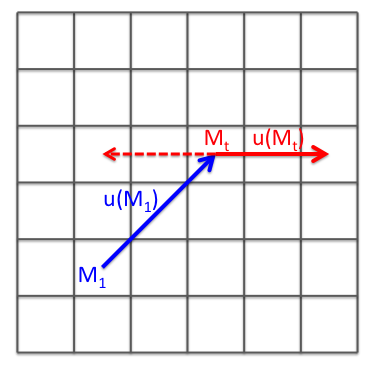
\includegraphics[height=5cm]{figures/fig-invert-trsf.png}
\end{center}
\caption{\label{fig:invert:transformation}$M_t$ is $M_1$ transformed by $T_{t \leftarrow 1}$, i.e. $M_t = M_1 + \mathbf{u}_{t \leftarrow 1}(M_1) $ where $\mathbf{u}_{t \leftarrow 1}(M_1)$ is the blue vector. $T_{t \leftarrow 1}^{-1}$ at $M_t$ should then by defined by the opposite of this blue vector (so that $M_t$ can project on $M_1$). By building the inverse of $T_{t \leftarrow 1}$ with the opposite of the $\mathbf{u}_{t \leftarrow 1}$ vector field, $T_{t \leftarrow 1}^{-1}$ at $M_t$ would be defined by $- \mathbf{u}_{t \leftarrow 1}(M_t)$, i.e. the dashed red vector (and thus not equal to $- \mathbf{u}_{t \leftarrow 1}(M_1)$, the opposite of the blue vector). This can be an acceptable approximation iff $\mathbf{u}_{t \leftarrow 1}(M_t)$ (the red vector) is sufficiently similar to $\mathbf{u}_{t \leftarrow 1}(M_1)$ (the blue vector).}
\end{figure}

$M_t$ is partway on the "line" joining $M_0$ and $M_1$ and at a "distance" $t$   from $M_1$ and $(1-t)$ from $M_0$. 
We have then
\begin{eqnarray*}
M_t =  (1-t) M_0 + t M_1 
& \Leftrightarrow &
 M_0 = \frac{1}{1-t} M_t - \frac{t}{1-t} M_1 \\
& \Leftrightarrow &
 M_0
 = \frac{1}{1-t} M_t - \frac{t}{1-t} T_{1\leftarrow t} M_t \\
& \Leftrightarrow &
 M_0
 = \frac{1}{1-t} M_t - \frac{t}{1-t} 
 \left( M_t + \mathbf{u}_{1 \leftarrow t}(M_t) \right) \\
 & \Leftrightarrow &
 M_0
 =  M_t - \frac{t}{1-t} 
 \mathbf{u}_{1 \leftarrow t}(M_t) \\
\end{eqnarray*}

The transformation $T_{0 \leftarrow t}$ is then represented by the vector field $\left(- \frac{t}{1-t}\mathbf{u}_{1 \leftarrow t}\right)$.

Finally, the image $I_t$ can be interpolated from the resampled $I_0$ and $I_1$ into $I_t$ frame, ie $I_0 \circ T_{0 \leftarrow t}$ and $I_1 \circ T_{1 \leftarrow t}$ with
\begin{displaymath}
I_t = (1-t) \times I_0 \circ T_{0 \leftarrow t}
+ t \times I_1 \circ T_{1 \leftarrow t}
\end{displaymath}




% \part{Developer documentation}

% 
\chapter{Registration procedure}

\section{\texttt{BAL\_PyramidalBlockMatching}}

\texttt{BAL\_PyramidalBlockMatching()}\footnote{\texttt{bal-blockmatching.c}} 
manages the hierarchical/pyramidal registration loop.

As input, it has the two images, $I_{ref}$ and $I_{flo}$, and two
transformations, $T_{left}$ and $T_{init}$. The registration consists
in computing $T_{res}$ such that $I_{flo} \circ T_{left} \circ
T_{res}$ can be superimposed onto $I_{ref}$. The computation of
$T_{res}$ is iterative and $T_{init}$ is the initialization of $T_{res}$


\subsection{Initialization}
\label{sec:devel:doc:trsfs:initialization}
The computation of
$T_{res}$ is iterative, its initial value, say $T$, depends on both
$T_{left}$ and $T_{init}$.
\begin{itemize}
\item if $T_{init}$ is given, $T = T_{init}$
\item else 
\begin{itemize}
\item if $T_{left}$ is given, $T = \mathbf{Id}$
\item $T$ is the translation that superimposes the
centers of the fields of view of the two images $I_{ref}$ and
$I_{flo}$ (computed by \texttt{BAL\_Compute\-ImageToImageTransformation()}\footnote{\texttt{bal-transformation-tools.c}}).
\end{itemize}
\end{itemize}



\subsection{Iterations over pyramid levels}

At each pyramid level $\ell$, images ${}^{(\ell)}I$ are computed with
the resampling transformation $T_{(\ell)} = T_{I \leftarrow
  {}^{(\ell)}I}$. This transformation is computed by
\texttt{BAL\_Compute\-ImageToImageTransformation()}\footnote{\texttt{bal-transformation-tools.c}}
(see also section \ref{sec:frame:resolution}).

A subsampled version of the reference image is computed by
${}^{(\ell)}I_{ref} = I_{ref} \circ T_{(\ell)}$. 
Let $T$ be the current estimation of the transformation, thus for the
level $\ell$, we will compute (with \texttt{BAL\_BlockMatching()}) a transformation with $T \circ
T_{(\ell)}$ as initial estimate. Of course, the returned result will
be composed by $T_{(\ell)}^{(-1)}$ afterwards.

Parameters for \texttt{BAL\_BlockMatching()} are then the subsampled
reference image ${}^{(\ell)}I_{ref} = I_{ref} \circ T_{(\ell)}$, the
floating image $I_{flo}$, the left handed transformation $T_{left}$
and the current estimate of the transformation $T \circ
T_{(\ell)}$ that allows to superimpose $I_{flo}$ onto
${}^{(\ell)}I_{ref}$, $I_{flo}$ being resampled by  
$I_{flo} \circ T_{left} \circ T \circ T_{(\ell)}$.

\section{\texttt{BAL\_BlockMatching}}

\texttt{BAL\_BlockMatching}\footnote{\texttt{bal-blockmatching.c}}
performs the registration for two given images $I_{ref}$ (note that
$I_{ref}$ can be a subsampled version of the original reference image)
and $I_{flo}$ (note that $I_{flo}$ is not subsampled, even if
$I_{ref}$ is), given the two transformations $T_{left}$ and $T^{(0)}$ 
which is the initial value for the transformation.

At each iteration $i$,
\begin{itemize}
\item resample $I_{flo}$ in the same geometry than $I_{ref}$, i.e. compute $I_{flo}^{(i)} = I_{flo} \circ T_{left} \circ T^{(i)}$
\item compute the incremental transformation from $I_{ref}$ to $I_{flo}^{(i)}$,
  i.e. $\delta T^{(i)} = T_{ I_{flo}^{(i)} \leftarrow I_{ref}}$
\item update the transformation $T^{(i+1)} = T^{(i)} \circ \delta T^{(i)}$
\end{itemize}




% \part{Developer notes}

% \chapter{\blockmatching versus \baladin}

\section{Blocks management}

There are two issues.

\begin{itemize}

\item The number of blocks calculated in the earlier versions of \baladin was erroneous (and may yield an overflow). 
\item As a consequence, some blocks (that should have been considered) were discarded.
\item the ordering of the blocks in the earlier versions of \baladin was $z$ varies first, then $y$ and finally $x$, so that the index of a block is given by $z + ( y + x * dim_y) * dim_z$. 

\end{itemize}

This behavior can be mimicked with the define \verb|_ORIGINAL_BALADIN_BLOCKS_MANAGEMENT_| in the latest version of \baladin (except for the overflow). 

It seems that the indexing order is important (experiments have been conducted by changing the indexing, with the same blocks being discarded), since results may numerically differ. It can be suspected (but has not be proven) that it may change the "best" pairing, because of the scan order, when several blocks result in the same criteria value.



\section{D\'efinition des blocs}

La dimension d'une image est $D$ (les coordonn\'ees des points vont de $0$ \`a $D-1$), on ne veut pas de blocs dans les $\textit{offset}_p$ premiers points, ni dans les $\textit{offset}_d$ derniers points. La dimension d'un bloc est $B$ 
et les blocs sont espac\'es de $S$. On a donc 
\begin{itemize}
\item coordonn\'ee du premier point inclus dans le bloc $i , i\geq 0$ : 
$$x_0 = \textit{offset}_p + i * S$$ 
Donc le point $x$ est le premier point (origine) d'un bloc si
$$(x - \textit{offset}_p) \% S = 0$$ 
(le reste de la division euclidienne est $0$), et l'indice du bloc est alors  
$$(x - \textit{offset}_p) / S$$
\item coordonn\'ee du dernier point inclus dans le bloc $i$ : 
$$x_1 = \textit{offset}_p + i * S + (B-1)$$
\end{itemize}
Pour qu'un bloc soit valide, il faut donc 
\begin{eqnarray*}
\textit{offset}_p + i * S + (B-1) \leq D - 1 - \textit{offset}_d
& \Longleftrightarrow &
i * S \leq D - 1 - \textit{offset}_d -B +1 - \textit{offset}_p \\
i * S \leq D-B - \textit{offset}_d - \textit{offset}_p
\end{eqnarray*}
Le dernier indice valide est donc 
$$
i_d = \left( D-B - \textit{offset}_d - \textit{offset}_p \right) / S
$$
Comme les indices commencent \`a $0$, il y a donc $i_d +1$ blocs avec
$$
i_d + 1 = \left( D-B - \textit{offset}_d - \textit{offset}_p \right) / S + 1
$$


% \part{Misc}

% 

\chapter{Misc}

\section{Calcul d'une transformation aux moindres carrées}

\subsection{Rappels}
\begin{eqnarray*}
\sum_i \left( x_i - \bar{x} \right)^2 
& = &
\sum_i \left( x_i^2 - 2 x_i \bar{x} + \bar{x}^2 \right) \\
& = &
\sum_i x_i^2 - 2 \bar{x} \sum_i x_i + N \bar{x}^2 \\
& = &
\sum_i x_i^2 - 2 \bar{x} N \bar{x} + N \bar{x}^2 \\
& = &
\sum_i x_i^2 - N \bar{x}^2 
\end{eqnarray*}

\begin{eqnarray*}
\sum_i \left( x_i - \bar{x} \right) \left( x'_i - \bar{x}' \right) 
& = &
\sum_i x_i x'_i - \bar{x} \sum_i x'_i - \bar{x}' \sum_i x_i + N \bar{x} \bar{x}' \\
& = &
\sum_i x_i x'_i - \bar{x} N \bar{x}' - \bar{x}' N \bar{x} + N \bar{x} \bar{x}' \\
& = &
\sum_i x_i x'_i - N \bar{x} \bar{x}'
\end{eqnarray*}

\subsection{Translation + scaling}

Le crit\`ere est de la forme
$$
\sum_i \left( a_x x_i + t_x - x'_i \right)^2 + \ldots
$$

La d\'eriv\'ee par rapport \`a $t_x$ donne
\begin{eqnarray*}
\sum_i \left( a_x x_i + t_x - x'_i \right) = 0
& \Longleftrightarrow &
a_x \sum_i x_i + N t_x - \sum_i x'_i = 0 \\
& \Longleftrightarrow &
t_x = \bar{x}' - a_x \bar{x} 
\end{eqnarray*}

La d\'eriv\'ee par rapport \`a $a_x$ donne
\begin{eqnarray*}
\sum_i x_i \left( a_x x_i + t_x - x'_i \right) = 0
& \Longleftrightarrow &
a_x \sum_i x_i^2 + t_x \sum_i x_i - \sum_i x_i x'_i = 0\\
& \Longleftrightarrow &
a_x \sum_i x_i^2 +
N \bar{x} \left( \bar{x}' - a_x \bar{x} \right) - \sum_i x_i x'_i = 0\\
& \Longleftrightarrow &
a_x \left( \sum_i x_i^2 - N \bar{x}^2 \right)
+ N \bar{x} \bar{x}' - \sum_i x_i x'_i = 0 \\
& \Longleftrightarrow &
a_x \sum_i \left( x_i - \bar{x} \right)^2  
 - \sum_i \left( x_i - \bar{x} \right)\left( x'_i - \bar{x}' \right) \\
& \Longleftrightarrow &
a_x = \frac{\sum_i \left( x_i - \bar{x} \right)\left( x'_i - \bar{x}' \right)}{\sum_i \left( x_i - \bar{x} \right)^2}
\end{eqnarray*}




\section{Notes}

\begin{itemize}

\item  la position du centre d'un bloc (cf CalculChampVecteur2D() et CalculChampVecteur3D()) est donn\'ee par 
$x = a + param->bl\_dx / 2.0$ avec $a$ origine du bloc, et $param->bl\_dx$ taille du bloc. Etant donn\'e que $a$ est au centre du bloc, il aurait fallu faire 
$x = a + (param->bl\_dx -1)/ 2.0$ !! [DONE]

\item dans CalculChampVecteur3D(), la taille du voisinage est de -$param->bl\_size\_neigh\_x$ a $+param->bl\_size\_neigh\_x$, et on parcourt le voisinage a partir de $a - param->bl\_size\_neigh\_x$ et en avan\c{c}ant de $param->bl_next_neigh_x$, ce qui fait que l'on ne teste pas forc\'ement le point central (ex: size = 3 et step = 2). A corriger.

\item Le calcul des r\'esidus devrait se faire par une distance de Mahalanobis. 
\begin{itemize}
\item Paires : $(M_i, M'_i)$
\item Transformation estim\'ee : $T = \arg \min \sum_i \| T \circ M_i - M'_i \|^2$
\item vecteurs r\'esidus : $\mathbf{r}_i = T \circ M_i - M'_i$
\item moyenne des r\'esidus : 
$\overline{\mathbf{r}} = \frac{1}{N} \sum_i \mathbf{r}_i$
\item matrice de covariance des r\'esidus : 
$C = \frac{1}{N} \sum_i (\mathbf{r}_i - \overline{\mathbf{r}}) (\mathbf{r}_i- \overline{\mathbf{r}})^T$
\item la distance de Mahalanobis s'\'ecrit 
$(\mathbf{r}_i- \overline{\mathbf{r}})^T C^{-1} (\mathbf{r}_i- \overline{\mathbf{r}})$

\end{itemize}
Maintenant, il faudrait calculer la distance par rapport \`a un r\'esidu nul...





\item tools = outils, basic = allocation, initialisation, ...

\item transformation\_type n'a pas \`a \^etre dans les param\`etres de recalage, juste dans les param\`etres locaux du 'main'

\end{itemize}






\printindex


\end{document}